\chapter{Implementace kryptobota}
\label{chap:impl}

Hlavní cíl této diplomové práce spočívá v implementaci kryptobota. Tento kryptobot má vytvořená pravidla vycházející z předem provedené technické analýzy.
Pravidla se následně aplikují na reálný trh a bot provádí obchody. Jeho postup a stav lze uživatelský přívětivě pozorovat skrze webové stránky, případně jeho akce
zastavit, nebo dokonce kompletně opustit tržní pozici. Implementovaný kryptobot je schopen obchodovat na burze Binance, která je jedna z největších a nejpopulárnějších
světových burz.

\section{Fungování kryptobota}
Pro kompletní fungování je zapotřebí několika kroků. Každý z těchto kroků (znázorněné na obrázku~\ref{fig:bot-schema}) je vysoce důležitý a výpadek jakékoli části může
mít kritické dopady na fungování a potenciální ziskovost obchodování. Proto je každá část systému navržena
a implementována co nejrobustněji a počítá s možností nedostupných služeb, případně databáze. Prvním krokem, který bude popsán podrobněji je stahování dat, následuje
technická analýza. Z analýzy vycházejí příkazy k obchodování. Ty budou taktéž podrobněji popsány. Poslední krok je následná realizace příkazů, komunikace s burzou
a vyhodnocování výsledků obchodování (backtesting).

\begin{figure}[ht]
    \centering
    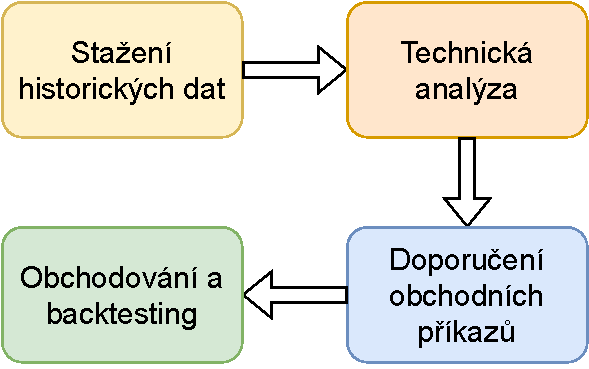
\includegraphics[width=0.8\textwidth]{Figures/bot-schema.pdf}
    \caption{Blokové schéma fungování kryptobota}
    \label{fig:bot-schema}
\end{figure}

\subsection{Historická data}
Úplným základem bota jsou historická data a jejich získávání je projektem jiného studenta. Burza Binance tato data poskytuje bezplatně a volně ke stažení, prakticky komukoli.
Lze si stáhnout svíčky,
jednotlivé obchody nebo agregované obchody. Svíčky jsou poskytovaný v granularitách od 1 vteřiny až po celý den. Z tohoto zdroje Binance zpřístupňuje data s jednodenním
zpožděním. Často však svíčky nejsou dostupné i několik dní, což zkresluje výsledky doporučení pro obchodování.
Pro potřebu bota v rámci této práce se stahují minutové svíčky se zmiňovaným jednodenním zpožděním. Důvod proč je toto dostačující je uveden dále v této práci.
Náležitě se musí ošetřit situace, kdy není server Binance dostupný nebo chybí data svicek kryptoměnového páru. Pokud k tomuto dojde, systém si zařadí do fronty svých úloh opětovnou
akci stažení potřebných dat. Jakmile jsou svíčky na lokálním serveru, provádí se importování do databáze. Po úspěšném zapsání do databáze následuje technická analýza.

\subsection{Technická analýza}
Fundamentální krok kryptobota je samotné provedení technické analýzy ve spolupráci s backtestingem. Z tohoto postupu vznikají nastavení obchodních příkazů, které jsou výhodné
a má smysl je obchodovat. Řešeni vytvořené v rámci je založené na rozboru kopců a dolin generovanými zavíracími cenami svíček. Kolísání cen nahoru a dolů by ve spojitém grafu
tvořilo čáru, ve kterých lze identifikovat lokální minima a maxima. Právě tyto lokální extrémy tvoří kopce a doliny. Cílem analýzy je pak odhalit kryptoměnové páry s dostatečně
velkým počtem těchto extrémů včetně velikosti jejich rozpětí. Jestliže by rozpětí růstu kopců bylo příliš malé, nemusely by být obchody dostatečně ziskové. Analýza kopců a dolin se takto
snaží odhalit dlouhodobě
ziskové páry. Proto nevadí, že se stahují a analyzují data s denní zpožděním. Toto řešení není založené na okamžité reakci, nýbrž na předpokladu dlouhodobé ziskovosti.

% TODO: Obrázek kopců a doliny s vizualizací nástupní a sestupní hrany
Scénář obchodování pro strategii kopců a dolin je následující: v momentě, kdy se dosáhlo minima, cena se odráží a začíná stoupat. Tím je započata nákupní fáze
se snahou uzavřít obchod s co nejnižší nákupní cenou. Další stoupání ceny je příznivou situací, během které se zhodnocuje investice. Dosáhnutím lokálního maxima se trend láme a začíná klesat
-- nastává prodejní fáze opět se snahou prodat, tentokrát za co nejvyšší cenu. Konkrétní realizace je pak popsána v sekci~\ref{subsec:exchanges-comm}.


\section{Datová struktura}
Fungování kryptobota je nejvíce závislé na 4 relacích. Jejich ER diagram lze vidět na obrázku \ref{fig:er-diag}. Jednotlivé popisy sloupců těchto tabulek se nacházejí v příloze této
práce (\ref{tab:tradeOrder}, \ref{tab:tradeOrderIteration}, \ref{tab:tradeOrderProgress}, \ref{tab:tradeOrderProgressPart}).

\begin{figure}[h]
    \centering
    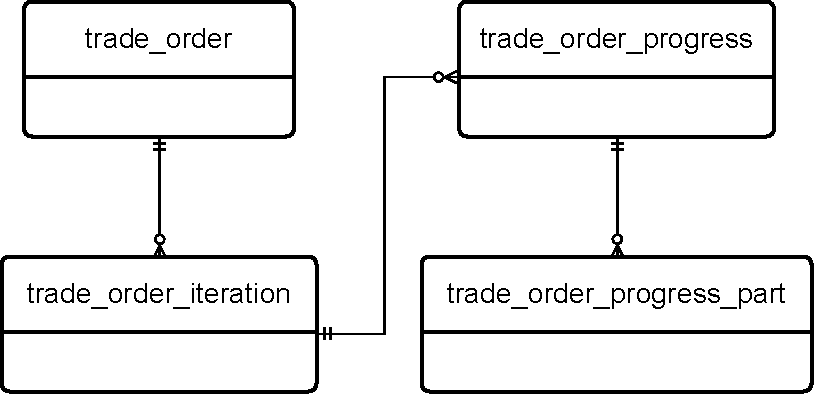
\includegraphics[width=0.8\textwidth]{Figures/er-trade-order.pdf}
    \caption{ER diagram důležitých entit}
    \label{fig:er-diag}
\end{figure}

Většina abstraktnější logiky rozhodování je obsažena v databázových procedurách. Tyto procedury jsou navíc volány taktéž triggery, případně periodicky v rámci databázové události (event), které
databázový systém MySQL nabízí. Na tabulky \emph{trade\_order\_iteration} a \emph{trade\_order\_progress} jsou navázány \emph{after insert} a \emph{after update} triggery. V momentě, kdy je vložen
nový záznam iterace, automaticky je skrze trigger zavolána procedura, která vytvoří nový záznam do tabulky \emph{trade\_order\_progress}. S touto tabulkou už pak pracuje \emph{Executioner}, který
příkaz zašle na burzu.

Jednotlivé části obchodu získávané \emph{Stream listenerem} se vkládají do tabulky \emph{trade\_order\_progress\_part}. I pro tuto tabulku existuje after insert trigger. Jakmile je detekován
záznam ohledně ukončení obchodu, korektně se zaktualizuje související záznam z \emph{trade\_order\_progress}, spojený cizím klíčem. Po provedení aktualizace je opětovně volána procedura aktualizující
\emph{trade\_order\_iteration} a následně i samotná \emph{trade\_order}.


\section{Výběr párů a realizace obchodních příkazů}
\label{subsec:trade-orders}
Vytvoření obchodních příkazů je starostí předchozího kroku, zabývající se technickou analýzou. Ovšem počet způsobů, jak tyto příkazy vytvořit není pouze jeden a je závislý na konkrétním
nastavení. Pro analýzu kopců a dolin jsou nezbytně důležité dva parametry: velikosti vzestupu a sestupu. Ty zastávají procentuální změnu, o kterou se musí aktuální cena zvednout, nebo klesnout,
aby se situace v časovém okně označily jako dolina, respektive kopec. Díky těmto dvěma jednoduchým parametrům lze získat důležité informace o kryptoměnovém páru, konkrétně:
\begin{itemize}
    \item délka kopce,
    \item délka doliny,
    \item ziskovost jednotlivých stoupání.
\end{itemize}
Společně z dat získaných ze svíček (počet obchodů, objemy obchodů, \ldots) a statisticky dopočtených dat (medián a průměr objemu obchodů) se vydolují další rozhodující   informace.
Těmi je poměr počtu obchodů, poměr velikost objemu obchodů a počet obchodů vykonaných za den. Během backtestingu se simuluje obchodování o velikosti mediánu obchodů. Jestliže
algoritmus odhalí například 200 kopců během jednoho dne, znamenalo by to vykonání 200 obchodů. Toto číslo se dá do poměru s celkovým počtem vykonaných obchodů na kryptoměnovém páru.
Obdobně se získá poměr velikosti objemů jednotlivých obchodů. Tyto poměry, společně s celkovým počtem obchodů, jsou důležité z pohledu ovlivňování trhu a zachování likvidity.
Pokud by velikost těchto poměrů byla příliš velká, bylo by obchodování daného kryptoměnového páru riskantní, jelikož každý obchod kryptobota by mohl výrazně ovlivnit situaci na trhu
a způsobovat výkyvy ceny. Zároveň by obchody nemusely být vypořádány, jednoduše protože by se trh stával nelikvidním a rozpětí mezi poptávkou a nabídkou by se rozšířilo.

Informace o délce kopců a dolin slouží jako pomocník pro nastavení maximální doby, po kterou se má bot pokoušet nakoupit. A samozřejmě, ziskovost slouží jako hlavní indikátor
pro výběr páru, které je doporučeno obchodovat. Ovšem ziskovost záleží na vybraném stylu obchodování a opakování příkazu, které si zaslouží podrobnější popis.

\subsection{Opakování příkazu}
Samotný příkaz se skládá z několika opakování, neboli iterací (obrázek \ref{fig:trade-order-parts}). Každá iterace má 2 fáze -- nákupní a prodejní. Pro úplnost je ještě nutné definovat, co znamená ukončení jedné iterace.
\begin{figure}[ht]
    \centering
    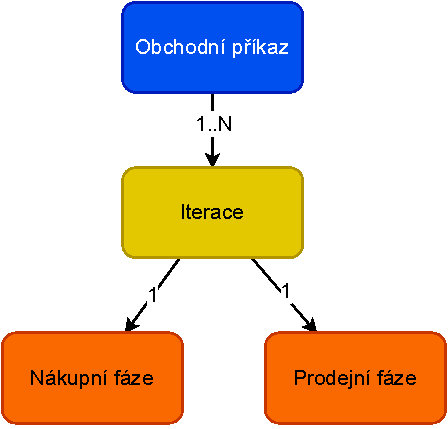
\includegraphics[width=0.5\textwidth]{Figures/trade-order-parts.pdf}
    \caption{Dělení obchodního příkazu}
    \label{fig:trade-order-parts}
\end{figure}
Ukončení iterace nastává ve 2 případech:
\begin{enumerate}
    \item nepovedla se nákupní fáze (tj. nic se nekoupilo),
    \item ukončila se prodejní fáze.
\end{enumerate}
Prodejní fáze je uzavřena opět ve 2 situacích:
\begin{enumerate}
    \item úspěšný prodej,
    \item překročením maximální doby prodeje a prodej zbývajících aktiv příkazem typu \textsc{market}.
\end{enumerate}

Existují 2 řešené postupy pro opakování příkazů. Prvních z nich je opakování v sekvenci (obrázek \ref{subfig:sequence}), kdy se před začátkem iterace $n_i$ čeká na ukončení iterace $n_{i - 1}$, přičemž $i$ je pořadové
číslo iterace. Výhodou tohoto přístupu je jednoduché sledování aktuálního stavu otevřené pozici na trhu. Avšak nevýhoda je šance na zanedbání dlouhého kopce a nevyužití případné ziskové situace.
Proto byla vymyšlena druhá metoda opakování.

\begin{figure}[ht]
    \centering
    \subfloat[\centering Opakování obchodu v sekvenci]{{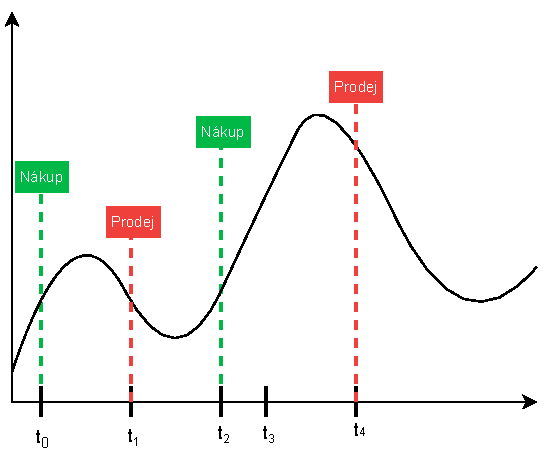
\includegraphics[width=0.45\textwidth]{Figures/sequence.pdf}}\label{subfig:sequence}}
    \qquad
    \subfloat[\centering Opakování obchodu v kaskádě]{{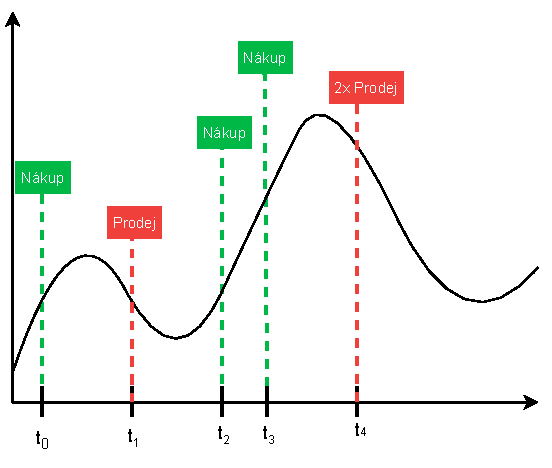
\includegraphics[width=0.45\textwidth]{Figures/cascade.pdf}}\label{subfig:cascade}}

    \subfloat[\centering Opakování v sekvenci - časová osa]{{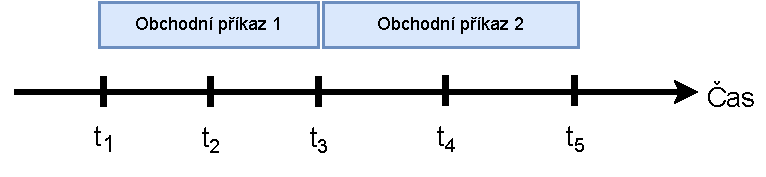
\includegraphics[width=0.45\textwidth]{Figures/sekvence-timeline.pdf}}\label{subfig:sequence-timeline}}
    \qquad
    \subfloat[\centering Opakování v kaskádě - časová osa]{{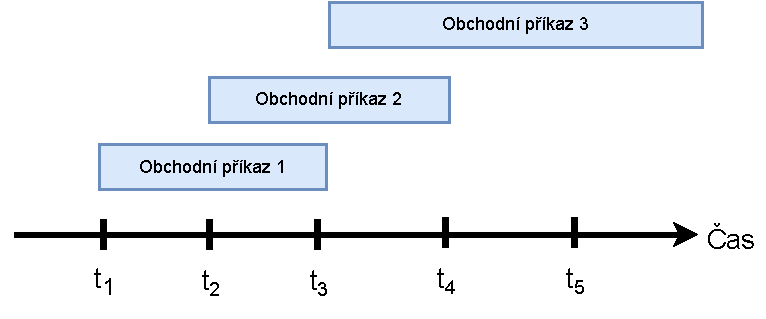
\includegraphics[width=0.45\textwidth]{Figures/kaskada-timeline.pdf}}\label{subfig:cascade-timeline}}
    \caption{Strategie opakování obchodu}
    \label{fig:trade-repeat}
\end{figure}

Schopnost obchodovat iterace v kaskádě (\ref{subfig:cascade}) s sebou přináší řešení na dlouhé kopce, ve kterých cena roste delší dobu. Kaskáda se oproti sekvenci liší v možnosti spuštění
následujícího opakování příkazu
už v momentě, kdy je úspěšně ukončena nákupní fáze iterace předchozí. V rámci tohoto postupu může docházet k více otevřeným pozicím na trhu. Nevýhodou je opět eventuální otevření pozice těsně před koncem stoupání
kopce. Jelikož se následně čeká na procentuální \enquote{propad} ceny dolů, je vysoká pravděpodobnost, že tato pozice bude prodělečná. Další nežádoucí situací je příliš rychlé otevírání
nových pozic a musí se stanovit limit buďto časově nebo maximálním počtem otevřených pozic v kaskádě. Bot v tomto případě podporuje obě možnosti.

\subsection{Způsoby obchodování}
Implementovaný kryptobot rozlišuje 2 způsoby obchodování, a to fixní a složené úročení. Fixní způsob otevírá pozice vždy na stejnou obchodovanou částku. Ve své podstatě se jedná o jakýsi DCA. Pokud se
povede utržit zisk, je již \enquote{odložen mimo}. V případě ztráty v obchodě je nutné ji kompenzovat, ať už ze získaných zisků nebo ze zásob.
Složené úročení, jak již název napovídá, reinvestuje vše, hodnotu původního vkladu zvýšenou o zisk nebo sníženou o ztrátu z předchozí iterace.
Účelem je takto maximalizovat zisk. Ovšem tento styl obchodování s sebou přináší riziko ovlivňování trhu. Jestliže
by investovaná částka narostla do velkých objemů může obchod způsobit ovlivnění tržní ceny a snížit likviditu trhu. Proto je nutné tento složené úročení limitovat maximální investovanou částkou.


\subsection{Skutečné obchodní příkazy}
Obchodování na základě kopců a dolin je pro burzy naprosto irelevantní. Burzy přijímají pouze příkazy popsané v části~\ref{subsec:market-trade-orders}. Nezbytností je tedy napárovat scénáře
obchodování na kombinací s těmito příkazy.

Zachycení začátku vzestupného trendu a tedy i začínajícího kopce se dá realizovat jednoduše s použitím příkazu \textsc{trailing stop-limit}. Důležitý
je právě onen \emph{trailing}, který počítá procentuální změnu tržní ceny. Problémové může být krátkodobé zachvění ceny, které by způsobilo zařazení příkazu do orderbooku, ale ve skutečnosti
by trh pokračoval v klesajícím trendu. Možnost, jak se tomuto jevu vyvarovat nabízí nepovinná \emph{stop} neboli \enquote{aktivační} cena. Teprve v momentě, kdy je proražena stop cena se začíná počítat trailing
delta. Avšak v této situaci nastává komplikace s reálnou burzou: stop cena a limitní cena nelze zadat jako procento aktuálního kurzu, ale musí to být konkrétní hodnoty. Pokud by v nákupní fázi
byla použita stop cena, může dojít k okolnostem, během kterých tržní cena výrazně klesne. Jakmile se odrazí a tržní cena opět stoupne, nedojde k nákupu, neboť se čeká, dokud se neprotne hranice
aktivační ceny. Nejenže by nákup trval dlouhou dobu, ale výrazná část kopce by se \enquote{ignorovala} a to rozhodně není žádoucí. Přestože bot poskytuje možnost nakoupit příkazy typu \textsc{market,
    limit, trailing stop-limit}, skutečně se používá pouze \textsc{trailing stop-limit} bez použití aktivační ceny.

Realizace prodejní fáze se potýká s podobnými problémy. Při použití příkazu \textsc{trailing stop-limit} bez aktivační ceny může dojít k drobnému záchvěvu ceny a předčasnému prodeji, což může
vést ke ztrátovému obchodu. Naopak pokud se použije aktivační cena, může dojít k rychlému skoku do klesajícího trendu, aktivační cena nebude nikdy proražena a prodejní fáze bude ukončena na základě
časového limitu s obrovskou ztrátou. Existuje ještě jedna střední cesta a tím je příkaz \textsc{OCO} (\enquote{One-Cancels-the-Other}). Jedná se vlastně o kombinaci dvou příkazů, \textsc{limit} a
\textsc{stop limit}. \textsc{OCO} příkaz je speciální v tom, že pokud je 1 příkaz jakkoli ukončen (vyplněním nebo zrušením), automaticky je zrušen i příkaz související.
V tomto případě \textsc{limit} zastřešuje horní hranici, nad
kterou dojde k prodeji a \textsc{stop limit} spodní hranici v případě pádu tržní ceny. Vytvořený bot umí využít těchto \textsc{OCO} příkazů v maximální prospěch periodickým kontrolováním tržní ceny
a vlastním přepočtem procentuální změny. Pokud se cena dostatečně zvýší, zruší momentálně nastavený \textsc{OCO} příkaz a zadá nový s cenami posunutými nahoru. K prodeji pak dojde pouze v případě poklesu tržní
ceny na hranici příkazu \textsc{stop limit} nebo pokud by kryptobot zasáhl výpadek. Teto metodě využití \textsc{OCO} příkazů přezdívá autor zajištěné obchodování, neboli taky \emph{peaking}.

\subsubsection{Platnost příkazu}
Binance neposkytuje maximální dobu platnosti příkazu ve smyslu předání časového razítka vypršení platnosti nebo maximální doby trvání. Jelikož příkazy mohou být vyplněny jen částečně, existují
3 nastavení času platnosti:
\begin{enumerate}
    \item Good-Till-Cancel (GTC),
    \item Immediate-Or-Cancel (IOC),
    \item Fill-Or-Kill (FOK).
\end{enumerate}
Tyto nastavení se nevztahují na příkazy typu \textsc{market}. Příkaz s platností GTC bude platný tak dlouho, dokud nebude objednávka kompletně vyplněna (nakoupen nebo prodán celý požadovaný objem aktiv)
nebo zrušena uživatelem. Oproti tomu v
režimu IOC se matching engine pokusí ihned alespoň částečně vypořádat objednávku na limitní cenové hladině s obchodovaným množstvím. Pokud se vyplní kompletní obchod, nic dalšího
se neděje. V případě částečného vypořádání je zbytek příkazu zrušen. Pokud na zadané cenové hladině není dostupné žádné obchodovatelné množství, je příkaz ihned zrušen.
Poslední a zároveň nejpřísnější doba vypršení FOK vyžaduje okamžité plné zobchodování příkazu. Jestliže tomuto nemůže trh vyhovět, je příkaz stornován.

Režim FOK je pro implementovaného kryptobota zbytečně přísný. Odzkoušeny byly režimy GTC a IOC, ale nepřinesly žádné velké rozdíly. Avšak to může být způsobeno malým objemem obchodovaného aktiva.
V případě, kdy by bot obchodoval značně vyšší částky, byly by rozdíly v režimech platnosti příkazů znatelnější. V tomto případě se nabízí upřednostnit spíše platnost IOC, aby byly příkazy
vypořádány dostatečně rychle.

\section{Komunikace s burzou Binance}
\label{subsec:exchanges-comm}
Přestože většina logiky kryptobota je realizovaná v databázi pomocí uložených procedur a funkcí, nelze všechno takto provést. Obchodní příkazy kryptobota obsahují abstrakci, kterou je
nutné převést na reálné hodnoty, především limitní a aktivační ceny. Komunikace s burzou probíhá s pomocí dvou samostatných komponent. Obě mají trochu jiný účel a zaslouží si vlastní krátkou sekci.
Předtím, než se popíšou tyto komponenty, bude čtenáři přiblíženo API burzy Binance. \cite{binance:docs}

\subsection{Binance API}
Binance poskytuje aplikační rozhraní přes protokol HTTPS a do budoucna se chystá i rozhraní založené na websocketech.
Pro komunikace si uživatel musí zajistit dvojici klíčů, \emph{API} klíč
a \emph{secret} klíč.
Základní URL pro zasílání požadavků je \verb|https://api.binance.com|.
Všechny potřebné informace ke koncovým bodům rozhraní jsou popsány v dokumentaci, avšak pro potřeby kryptobota bude zde přiblíženo jak rozhraní obecně, tak i pár konkrétních koncových bodů.

\subsubsection{Zabezpečení}
API klíčů může mít uživatel klidně více a skrze webové rozhraní lze na každý klíč nastavit jiná práva a omezení na konkrétní IP adresy. Tedy pokud uživatel zašle požadavek z jiné IP adresy než-li
té, která je zadané v systému, nebude Binance takovýto požadavek registrovat a odpoví chybovým hlášením. Navíc si Binance chrání své rozhraní omezením počtu volání koncových bodů (rate limiting). Tato omezení
jsou platná buďto na IP adresy nebo na identifikátor účtu uživatele.

Pro citlivé koncové body, které vykonávají akce na burze (vytváření příkazů, detail zůstatku, výběry, \ldots) vyžaduje API 2 zabezpečující prvky:
\begin{enumerate}
    \item HTTP požadavek musí obsahovat hlavičku \verb|X-MBX-APIKEY|,
    \item Součástí požadavku musí být parametr \verb|signature|
\end{enumerate} .
Obsahem hlavičky \verb|X-MBX-APIKEY| je uživatelův API klíč. Druhé je nutnost přiložení parametru \verb|signature|, což je zpráva zajišťující kryptografickou autentizace na základě
algoritmu \verb|HMAC-SHA256|. Jako klíč této do tohoto algoritmu vstupuje uživatelův \emph{secret} klíč, hodnotou je pak počet zasílaných parametrů.
Poslední ochranou je ochrana časová. Dalším parametrem, nazvaný \verb|recvWindow|, uživatel určuje jak dlouho (v milisekundách) je požadavek platný. V každém požadavku na API je přiloženo
časové razítko. Pokud server Binance nestihne vykonat požadavek v zadaném časovém okně, je celý požadavek zamítnut.

\subsubsection{Popis koncových bodů}
Koncové body mohou občas podporovat více parametrů, než jaké kryptobot reálně používá. Pro lepší přehlednost budou uvedeny a popsány parametry, které jsou reálně využity. Návratové zprávy získávané
při odpovědích budou taktéž popsány v potřebné míře.

\paragraph*{Nový příkaz}
Nejzákladnější a nejčastěji volaný koncový bod rozhraní slouží k vytvoření nového příkazu na burze. Botem využívané parametry jsou popsány v tabulce~\ref{tab:binance:new-order}.
\newline
\verb|POST /api/v3/order|
\begin{center}
    \begin{longtable}[h]{|l|C{4cm}|C{4cm}|m{4cm}|}
        \hline
        Parametr         & Povinný                                                                                         & Typ                                           & Popis                                  \\
        \hline
        \hline
        symbol           & \tikzcmark                                                                                      & Řetězec                                       & Název páru                             \\
        \hline
        side             & \tikzcmark                                                                                      & ENUM(buy, sell)                               & Nákup, prodej                          \\
        \hline
        type             & \tikzcmark                                                                                      & ENUM(\textsc{limit, market, stop loss limit}) & Typ příkazu                            \\
        \hline
        timeInForce      & \textsc{limit, stop loss limit, take profit limit}                                              & ENUM(gtc, ioc, fok)                           & Platnost příkazu                       \\
        \hline
        quantity         & \textsc{limit, market, stop loss, stop loss limit, take profit, take profit limit, limit maker} & Desetinný                                     & Množství base měny k nakoupení/prodeji \\
        \hline
        price            & \textsc{limit, stop loss limit, take profit limit, limit maker}                                 & Desetinný                                     & Cena                                   \\
        \hline
        stopPrice        & \textsc{stop loss, stop loss limit, take profit, take profit limit}                             & Desetinný                                     & Aktivační cena                         \\
        \hline
        trailingDelta    & \textsc{stop loss, stop loss limit, take profit, take profit limit}                             & Celočíselný                                   & Změna od extrému                       \\
        \hline
        newOrderRespType & \tikzxmark                                                                                      & ENUM(ack, result, full)                       & Velikost odpovědi                      \\
        \hline
        \caption{Parametry pro zadání nového příkazu}
        \label{tab:binance:new-order}
    \end{longtable}
\end{center}
Velikost odpovědi serveru burzy se dá nastavit ve 3 režimech v tomto pořadí od nejmenší po největší: \verb|ACK, RESULT, FULL|. Implementovaný kryptobot konkrétně využívá režim
odpovědi \verb|RESULT|. Odpověď tedy přichází ve formátu znázorněn v kódu~\ref{src:newOrder}.

\lstinputlisting[label=src:newOrder,caption={Odpovědi založení nového příkazu}]{Sources/new_order.json}

\paragraph*{Zrušení příkazu}
Další často využívaný koncový bod. Zrušení nastává, pokud příkaz přesáhne svou maximální dobu trvání na straně bota. Parametry
pro ukončení příkazu jsou v tabulce~\ref{tab:binance:cancel-order}
\newline
\verb|DELETE /api/v3/order|
\begin{center}
    \begin{longtable}[h]{|l|C{4cm}|C{4cm}|m{4cm}|}
        \hline
        Parametr          & Povinný                        & Typ         & Popis                \\
        \hline
        \hline
        symbol            & \tikzcmark                     & Řetězec     & Název páru           \\
        \hline
        orderId           & orderId nebo origClientOrderId & Celočíselný & ID příkazu           \\
        \hline
        origClientOrderId & orderId nebo origClientOrderId & Řetězec     & Klientské ID příkazu \\
        \hline
        \caption{Parametry pro zrušení příkazu}
        \label{tab:binance:cancel-order}
    \end{longtable}
\end{center}
Odpověď na požadavky zrušení příkazu kopírují formát při zadávání nových příkazů a je viditelný na~\ref{src:newOrder}.

\paragraph*{Nový OCO příkaz}
Metoda zajištěného obchodování, nazvaná taky \emph{peaking}, využívá právě OCO příkazů pro kontrolu spodní i horní hranice při změně kurzu kryptoměnového páru.
Parametry, které kryptobot nastavuje jsou v tabulce~\ref{tab:binance:new-oco}.
\newline
\verb|POST /api/v3/order/oco|
\begin{center}
    \begin{longtable}[h]{|l|c|c|m{3.7cm}|}
        \hline
        Parametr             & Povinný                 & Typ                 & Popis                                     \\
        \hline
        \hline
        symbol               & \tikzcmark              & Řetězec             & Název páru                                \\
        \hline
        side                 & \tikzcmark              & ENUM(buy, sell)     & Nákup, prodej                             \\
        \hline
        quantity             & \tikzcmark              & Desetinný           & Množství base měny k nakoupení/prodeji    \\
        \hline
        price                & \tikzcmark              & Desetinný           & Cena                                      \\
        \hline
        stopPrice            & \tikzcmark              & Desetinný           & Aktivační cena \textsc{stop loss} příkazu \\
        \hline
        stopLimitPrice       & \tikzxmark              & Desetinný           & Limitní cena \textsc{stop loss} příkazu   \\
        \hline
        stopLimitTimeInForce & Pokud je stopLimitPrice & ENUM(gtc, ioc, fok) & Platnost příkazu \textsc{stop loss}       \\
        \hline
        trailingDelta        & \tikzxmark              & Celočíselný         & Změna od posledního extrému               \\
        \hline
        \caption{Parametry pro vytvoření nového OCO příkazu}
        \label{tab:binance:new-oco}
    \end{longtable}
\end{center}

Odpověď na zaslaný příkaz je ve formátu JSON zobrazen na~\ref{src:newOCO}.

\lstinputlisting[label=src:newOCO,caption={Obsah odpovědi na zrušení OCO příkazu}]{Sources/new_oco.json}

\paragraph*{Zrušení OCO příkazu}
Pokud při použití zajištěného obchodování se cena posouvá pozitivně pro aktuální stranu obchodu (myšleno nákup nebo prodej), kryptobot zruší platný OCO příkaz
na burze a nahradí ho novým. Pro zrušení OCO příkazu je poslán HTTP požadavek na následující koncový bod s parametry uvedenými v tabulce~\ref{tab:binance:cancel-oco}.
\newline
\verb|DELETE /api/v3/orderList|
\begin{center}
    \begin{longtable}[h]{|l|C{4cm}|c|m{3.7cm}|}
        \hline
        Parametr          & Povinný                            & Typ         & Popis                \\
        \hline
        \hline
        symbol            & \tikzcmark                         & Řetězec     & Název páru           \\
        \hline
        orderListId       & orderListId nebo listClientOrderId & Celočíselný & ID příkazu           \\
        \hline
        listClientOrderId & orderListId nebo listClientOrderId & Řetězec     & Klientské ID příkazu \\
        \hline
        \caption{Parametry pro zrušení OCO příkazu}
        \label{tab:binance:cancel-oco}
    \end{longtable}
\end{center}
Získaná odpověď strukturou odpovídá stejné zprávě jako při zaslání nového OCO příkazu, lze ji tedy vidět výše v kódu~\ref{src:newOCO}.

\paragraph*{Průměrná cena}
Získávání průměrné tržní ceny se využívá pro zajištěné a nezajištěné obchodování. Vyžaduje pouze jediný parametr, jak lze vidět na tabulce~\ref{tab:binance:avg-price}.
\newline
\verb|GET /api/v3/avgPrice|
\begin{center}
    \begin{longtable}[h]{|l|C{4cm}|c|m{3.7cm}|}
        \hline
        Parametr & Povinný    & Typ     & Popis      \\
        \hline
        \hline
        symbol   & \tikzcmark & Řetězec & Název páru \\
        \hline
        \caption{Parametry pro získání průměrné ceny}
        \label{tab:binance:avg-price}
    \end{longtable}
\end{center}
Odpověď lze vidět na~\ref{src:avgPrice}.

\lstinputlisting[label=src:avgPrice,caption={Odpověď na požadavek průměrné ceny}]{Sources/avg_price.json}

\subsubsection{Tržní pravidla}
Každý kryptoměnový pár na burze Binance má svou vlastní sadu obchodních pravidel sdružených do tzv \emph{filtrů}. Celkem může existovat až 13 filtrů pro každý pár, nicméně kryptobot na některé
pravidla nemůže nikdy narazit, jelikož nevyužívá například tzv. iceberg příkazy. V této práci tedy budou zahrnuta jen pravidla, na která bot musí reagovat.


\paragraph*{PRICE\_FILTER}
Definuje základní cenová pravidla při zadávání příkazů. Pokud hodnota pravidla (\ref{tab:binance:price_filter}) je rovna 0, tak se toto pravidla bere jako neaktivní a nemusí se na něj brát ohled.
\begin{center}
    \begin{longtable}[h]{|l|l|l|}
        \hline
        Název pravidla & Význam                                     & Splnění pravidla           \\
        \hline
        minPrice       & Minimální povolená cena                    & $ cena \geq  minPrice $    \\
        \hline
        maxPrice       & Maximální povolená cena                    & $ cena \leq maxPrice $     \\
        \hline
        tickSize       & Interval, o který lze měnit zadávanou cenu & $price \bmod tickSize = 0$ \\
        \hline
        \caption{Pravidla cenového filtru}
        \label{tab:binance:price_filter}
    \end{longtable}
\end{center}

\paragraph*{PERCENT\_PRICE}
I tento filtr, jako předchozí, upravuje příkazové cenové rozpětí, nicméně tento rozsah zakládá na průměrné ceně předchozích obchodů. Pravidla lze vidět v tabulce~\ref{tab:binance:percent_price}
\footnote{$WMA_{cena}$ označuje vážený klouzavý průměr ceny}.
\begin{center}
    \begin{longtable}[h]{|l|l|l|}
        \hline
        Název pravidla & Význam                               & Splnění pravidla                           \\
        \hline
        multiplierUp   & Násobitel horní hranice              & $ cena \leq multiplierUp * WMA_{cena} $    \\
        \hline
        multiplierDown & Násobitel spodní hranice             & $ cena \geq  multiplierDown * WMA_{cena} $ \\
        \hline
        avgPriceMins   & Počet minut, za které je počítán WMA &                                            \\
        \hline
        \caption{Pravidla procentuálního cenového filtru}
        \label{tab:binance:percent_price}
    \end{longtable}
\end{center}

\paragraph*{LOT\_SIZE}
Zadává platný rozsah obchodované kvantity neboli lotu. Jak projít tímto filtrem je vidět v tabulce~\ref{tab:binance:lot_filter}.
\begin{center}
    \begin{longtable}[h]{|l|l|l|}
        \hline
        Název pravidla & Význam                              & Splnění pravidla         \\
        \hline
        minQty         & Minimální povolený lot              & $ lot \geq minQty $      \\
        \hline
        maxQty         & Maximální povolený lot              & $ lot \leq  maxQty $     \\
        \hline
        stepSize       & Velikost, o kterou se smí lot měnit & $lot \bmod stepSize = 0$ \\
        \hline
        \caption{Pravidla velikosti lotu}
        \label{tab:binance:lot_filter}
    \end{longtable}
\end{center}

\paragraph*{MIN\_NOTIONAL}
Definuje minimální obchodovanou nominální hodnotu. Nominální hodnotou se rozumí součin ceny a lotu. Tento filtr je přednostně kontrolován vůči příkazům typu \textsc{limit}, nicméně
může být použit i na typ \textsc{market}. Jelikož při použití příkazu \textsc{market} se nezadává požadovaná cena, počítá se nominální hodnota s průměrnou cenou za posledních X minut
specifikovaných přesněji v pravidle (\ref{tab:binance:notional_filter}).
\begin{center}
    \begin{longtable}[h]{|l|l|l|}
        \hline
        Název pravidla & Význam                              & Splnění pravidla                \\
        \hline
        minNotional    & Minimální nominální hodnota         & $ cena * lot \geq minNotional $ \\
        \hline
        applyToMarket  & Platí i pro \textsc{market} příkazy &                                 \\
        \hline
        avgPriceMins   & Počet minut, za které je počítán MA &                                 \\
        \hline
        \caption{Pravidla nominální hodnoty}
        \label{tab:binance:notional_filter}
    \end{longtable}
\end{center}

\paragraph*{MAX\_NUM\_ALGO\_ORDERS}
Tento filtr upřesňuje maximální povolený počet aktivních \enquote{algo} příkazů na daný kryptoměnový pár. Algo příkazem se myslí konkrétně příkazy typu
\textsc{stop loss, stop loss limit, take profit, take profit limit}. OCO příkazy taktéž snižují uživatelovu kvótu na maximální počet algo příkazů.

\subsection{Executioner}
Komponenta executioner má na starosti obchodní příkazy. Konkrétně jejich zaslání na burzu a jejich zrušení a dohled na vlastní přepočet při použití metod zajištěného a nezajištěného obchodování. Komponenta
využívá asynchronní úlohy. Přepínání mezi těmito úlohami řídí modul \verb|asyncio| vytvoření právě pro asynchronní programování.

\subsubsection{Zaslání příkazu na burzu}
Kontrola zaslání příkazu se provádí periodicky, každých pár vteřin. Celý cyklus je znázorněn na aktivitním diagramu \ref{figure:sending-trade-order}.
Z databáze (tabulka \emph{trade\_order\_progress}) se načtou potřebné parametry příkazů. Následuje kontrola
dostatku volných prostředků (podkladová měna kryptoměnového páru). Jestliže není dostatek podkladové měny, konkrétní příkaz se neprovede a do databáze se zapíše chybný stav. V případě
úspěchu se pokračuje převedením procentuálních hodnot na reálné částky. Z burzy se skrze API stáhne aktuální kurz kryptoměnového páru, na jehož základě se dopočtou ony reálné částky, které
se chtějí obchodovat. Před závěrečným zasláním příkazu na burzu dochází k poslední kontrole a to na pravidla samotného trhu (minimální nominální hodnota, minimální kvantita, \ldots).
Konečně je příkaz odeslán pomocí REST API ke zpracování na Binance. Součástí odpovědi je pak jednoznačný identifikátor daného příkazu na Binance, ten se uloží do databáze. Tím končí jedna
iterace zasílání příkazu.

\begin{figure}
    \centering
    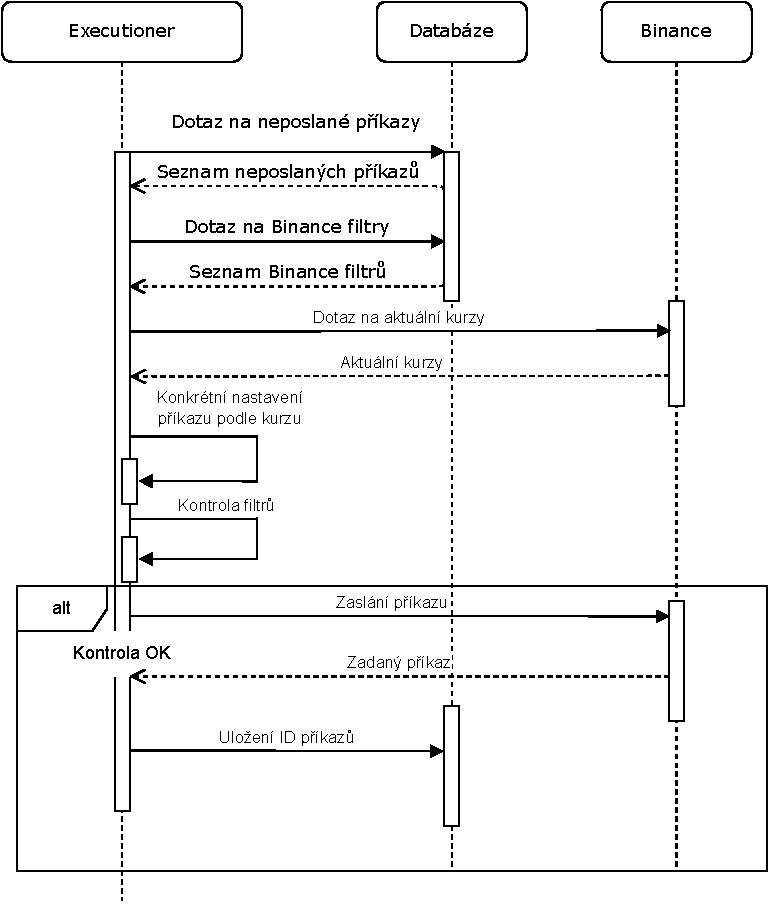
\includegraphics[width=0.7\textwidth]{Figures/Trading-bot-sequence.pdf}
    \caption{Aktivitní diagram zasílání příkazu}
    \label{figure:sending-trade-order}
\end{figure}

\subsubsection{Rušení příkazu}
Po zaslání příkazu na Binance je současně uloženo časové razítko, kdy byl příkaz odeslán. Opět, periodicky, se kontroluje překročení maximální doba trvání příkazu. Pokud se tato doba přesáhne,
je na Binance, přes API, zaslána žádost o zrušení toho příkazu. Pokud se jedná o prodejní příkaz, bot navíc reaguje vznikem nového příkazu pro okamžitý prodej přes \textsc{market}.

\subsubsection{Peaking}
Zvládnutí peakingu s sebou nese starost a vlastní přepočet změny kurzu. Tato změna se počítá od kurzu v momentě zasílání posledního příkazu. Peaking běží v rámci komponenty jako samostatná úloha.
Cyklicky v krátkých časových intervalech si stahuje z Binance momentální kurz kryptoměnového páru a spočítá procentuální přírůstek kurzu. Pouze v případě, že se jedná o pozitivní změnu vyšší než zadaná hranice, je
aktuální \textsc{OCO} příkaz zrušen a vytvořen nový s posunutými cenami nahoru. I v rámci této rychlé výměny příkazů se provádí stejné kontroly jako při normálním zasílání příkazu.

\subsubsection{Nezajištěné obchodování}
Metoda nezajištěného obchodování se snaží simulovat trailingové obchodování na straně kryptobota. Vlastní implementaci trailingu bot podporuje, jelikož ne všechny kryptoměnové burzy podporují tento typ příkazu.
Nevýhoda tohoto je vyšší náchylnost vůči selhání systému a to jak ze strany burzy tak i samotného kryptobota. Nicméně trailingové obchodování je důležitým nástrojem ziskového obchodování.

Samotná simulace trailingu je založená na počítání změny průměrného kurzu kryptoměnového páru. Byly vyzkoušeny dva přístupy:
\begin{enumerate}
    \item získání průměrné ceny skrze API Binance,
    \item vlastní průměrování kurzu.
\end{enumerate}
Důvodem průměrování je vyhlazování náhlých změn, které mohou být způsobeny obchody s velkým objemem.
V rámci prvního pokusu se bot periodicky dotazoval API Binance o získával informaci a průměrném kurzu daného páru. Pro většinu párů je tento průměr počítán za 5 minutové období. Tato skutečnost má za následek, že
je průměr příliš \enquote{pomalý}, tedy pomaleji reaguje na změny v aktuální tržní hodnotě. Důsledkem je dopad na ziskovost obchodů prováděných kryptobotem, jelikož obchodní příkaz je na burzu zadán pozdě.
Z tohoto důvodu bylo implementováno vlastní průměrování. Pomocí websocketů se kryptobot napojí na stream posílající zprávy o změně kurzu. Jakmile je obdrženo maximum zpráv (aktuálně nastaveno na 12) je
poslední zpráva zahozena a nová je přidána. Následně jsou přijaté kurzy zprůměrovány. Výsledný průměr je porovnán vůči poslednímu extrému. Překročí-li nastavenou procentuální změnu, je na burzu zaslán příkaz typu
\textsc{limit}, po jehož ukončení je fáze iterace ukončena.

Během testování a obchodování se druhý přístup vlastního průměrování ukázal jako ziskovější. To může být způsobeno právě rychlejší reakcí na změny tržní ceny kryptoměnového páru.

\subsection{Stream listener}
Úkolem stream listeneru je nepřetržité získávání zpráv o událostech od Binance. Vizuálně je proces naznačen na sekvenčním diagramu \ref{figure:listener}.
Spojení s burzou se navazuje pomocí technologie \emph{websocketů}. Ačkoli websockety nabízí možnost plně duplexní komunikace, Binance
neumožňuje zasílání příkazů přes tento komunikační kanál. Jedná se tedy pouze o pasivní naslouchání. Aby bylo spojení povoleno, je zapotřebí si vyžádat spojení se speciálním klíčem v URL parametru.
Tento klíč lze získat voláním REST API a je nutné ho nadále označovat za aktivní (taktéž voláním REST API). Z přicházejí zprávy o 3 událostech:
\begin{enumerate}
    \item aktualizace účtu,
    \item aktualizace zůstatku,
    \item aktualizace příkazu.
\end{enumerate}
Aktualizace účtu nastává v momentě, kdy se jakkoli změní zůstatek na účtu, např. zablokováním aktiv v rámci obchodování. Aktualizace zůstatku je zaslána, jakmile nastane vklad, výběr nebo převod z účtu.
Aktualizace příkazu, jak již název napovídá, je přijat při změně stavu příkazu způsobeným třeba zrušením příkazu, vypršením nebo vyplněním. Kryptobot reaguje na události týkající se aktualizací příkazů
a aktualizace účtu. Každá aktualizace příkazu je ihned uložena do databáze.

\begin{figure}
    \centering
    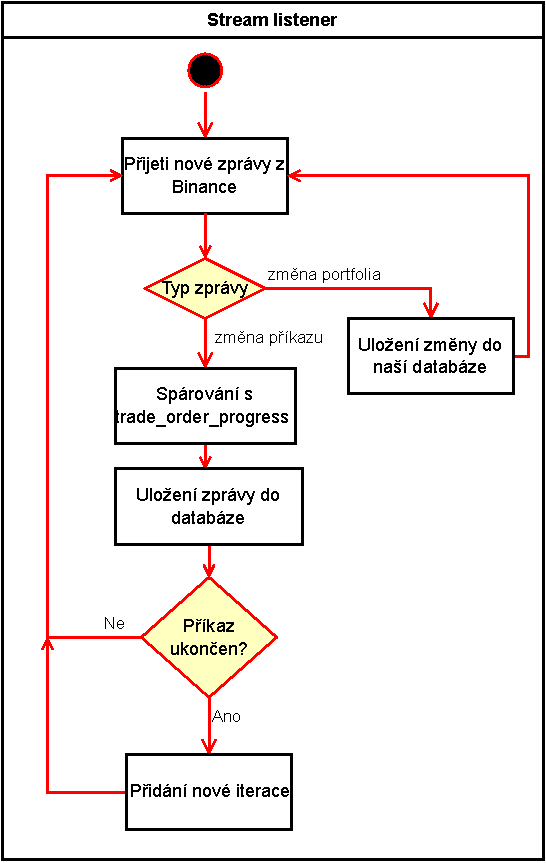
\includegraphics[width=0.7\textwidth]{Figures/listener.pdf}
    \caption{Sekvenční diagram komponenty Stream listener}
    \label{figure:listener}
\end{figure}

Aby bot měl dostupné vždy korektní informace provádí stream listener při svém spuštění kontrolu příkazů z databáze vůči burze. Pokud detekuje, že v databázi chybí nějaké informace z důvodu nějakého výpadku,
stáhne potřebná data skrze API a uloží je. Druhým opatřením, kterým stream listener disponuje, je ukládání zpráv do vyrovnávací paměti, pokud by došlo k výpadku databáze.


\section{Webové rozhraní}
Vytvořené webové rozhraní slouží k jednoduššímu posouzení aktuálního stavu kryptobota. Poskytuje 3 základní pohledy:
\begin{enumerate}
    \item pohled na stav obchodovaných kryptoměn a navržených párů z technické analýzy (obrázek~\ref{fig:web:market-dashboard}),
    \item pohled na stav databáze a běžících procesů (obrázek~\ref{fig:web:jobs-dashboard}),
    \item pohled na stav obchodních příkazu (obrázek~\ref{fig:web:trade-dashboard}).
\end{enumerate}
Zadávání nových příkazů je umožněno skrz formulář viditelný na obrázku~\ref{fig:web:new-order}. Uživatel jednoduše zadá název kryptoměnového páru, nastaví způsob opakování obchodů a způsob investice,
specifikuje dobu prodlev, maximální dobu trvání jednotlivých fází iterací, počet iterací a parametry obchodů. Výsledek obchodování je pak zobrazen na detailu obchodního příkazu (obrázek~\ref{fig:web:trade-order}).
Na detailech (obrázky \ref{subfig:web:desc}, \ref{subfig:web:iterations}, \ref{subfig:web:candles}) je pak postupně vidět konkrétní nastavení obchodního příkazu včetně celkových statistik ziskovosti, průběh jednotlivých
iterací včetně stavu konkrétních fází a nakonec svíčkový graf zaměřený na období, ve kterém byly prováděny obchody. Na svíčkovém grafu jsou rozsahové anotace vyjadřující ziskový nebo ztrátový obchod. Pro uživatele
webového rozhraní je tento graf interaktivní a může prohlížet jak si kryptobot se zadaným příkazem vedl.

\begin{figure}[b]
    \centering
    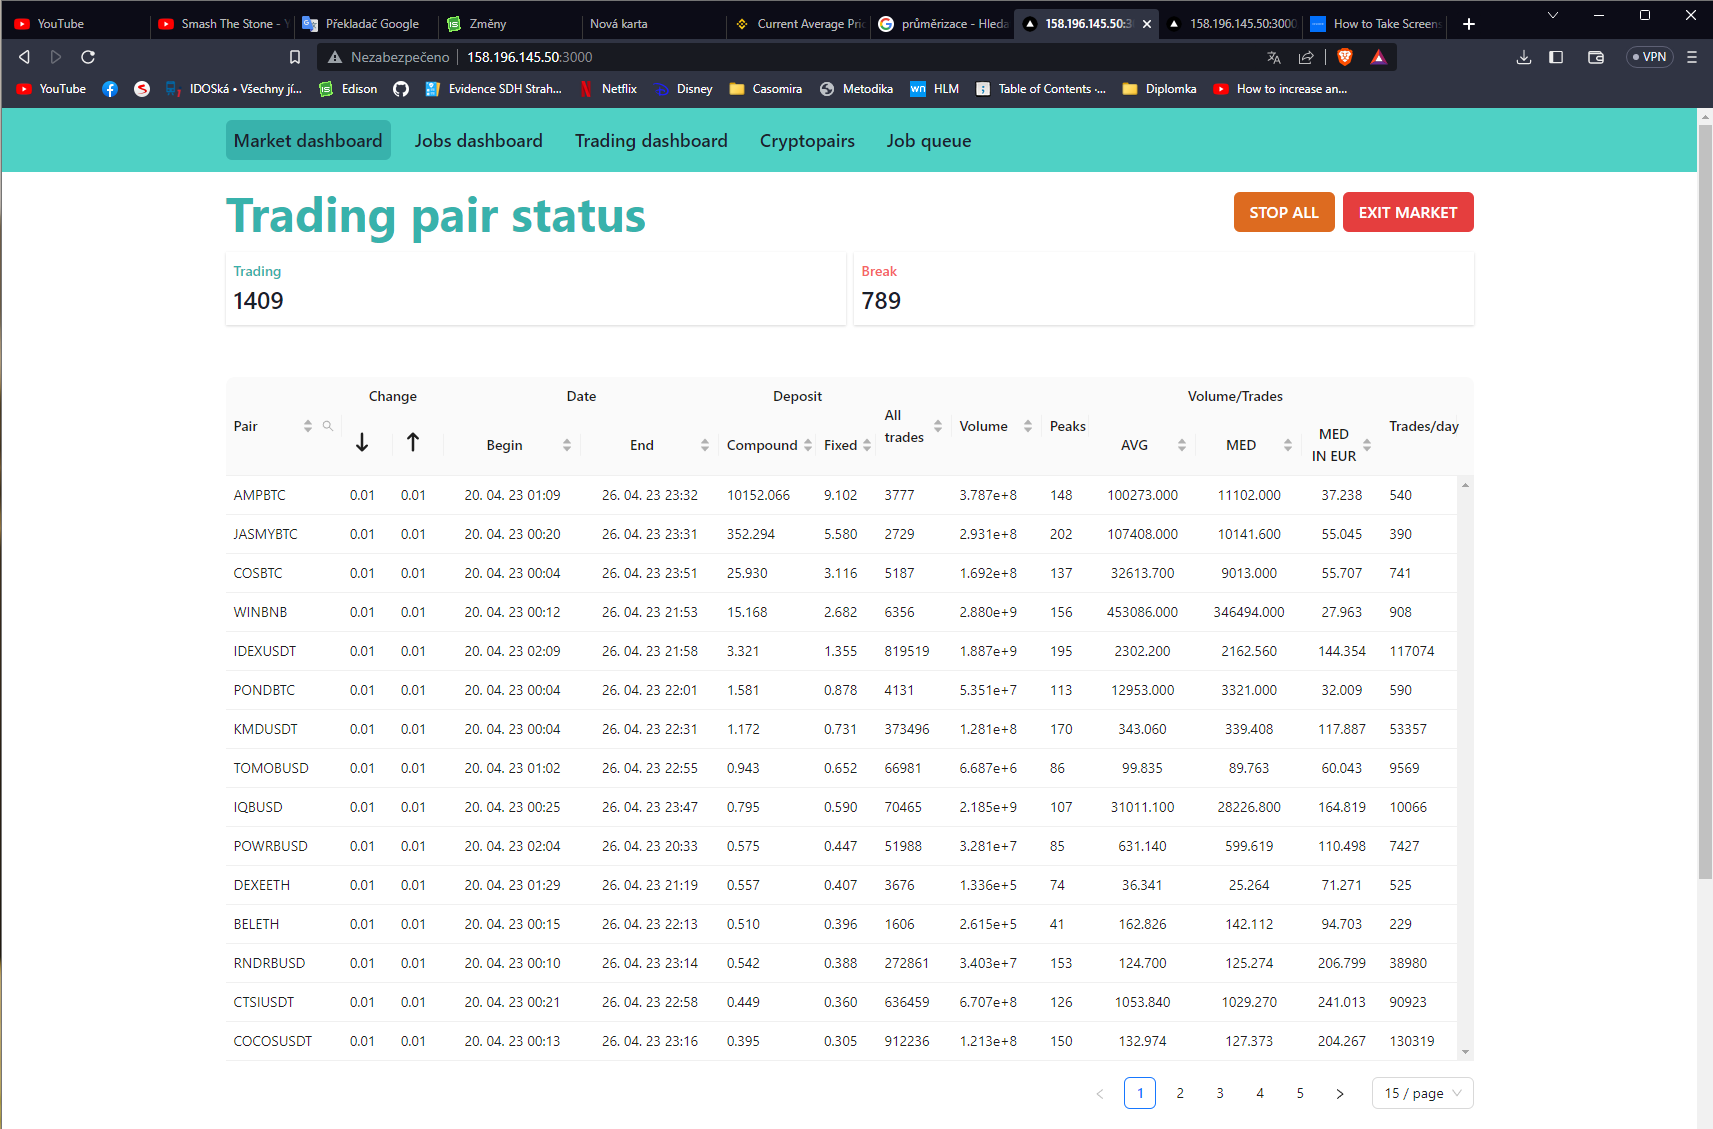
\includegraphics[width=0.6\textwidth]{Figures/web/market-dashboard.png}
    \caption{Stránka zobrazující stav kryptoměn a navržených párů}
    \label{fig:web:market-dashboard}
\end{figure}

\begin{figure}[b]
    \centering
    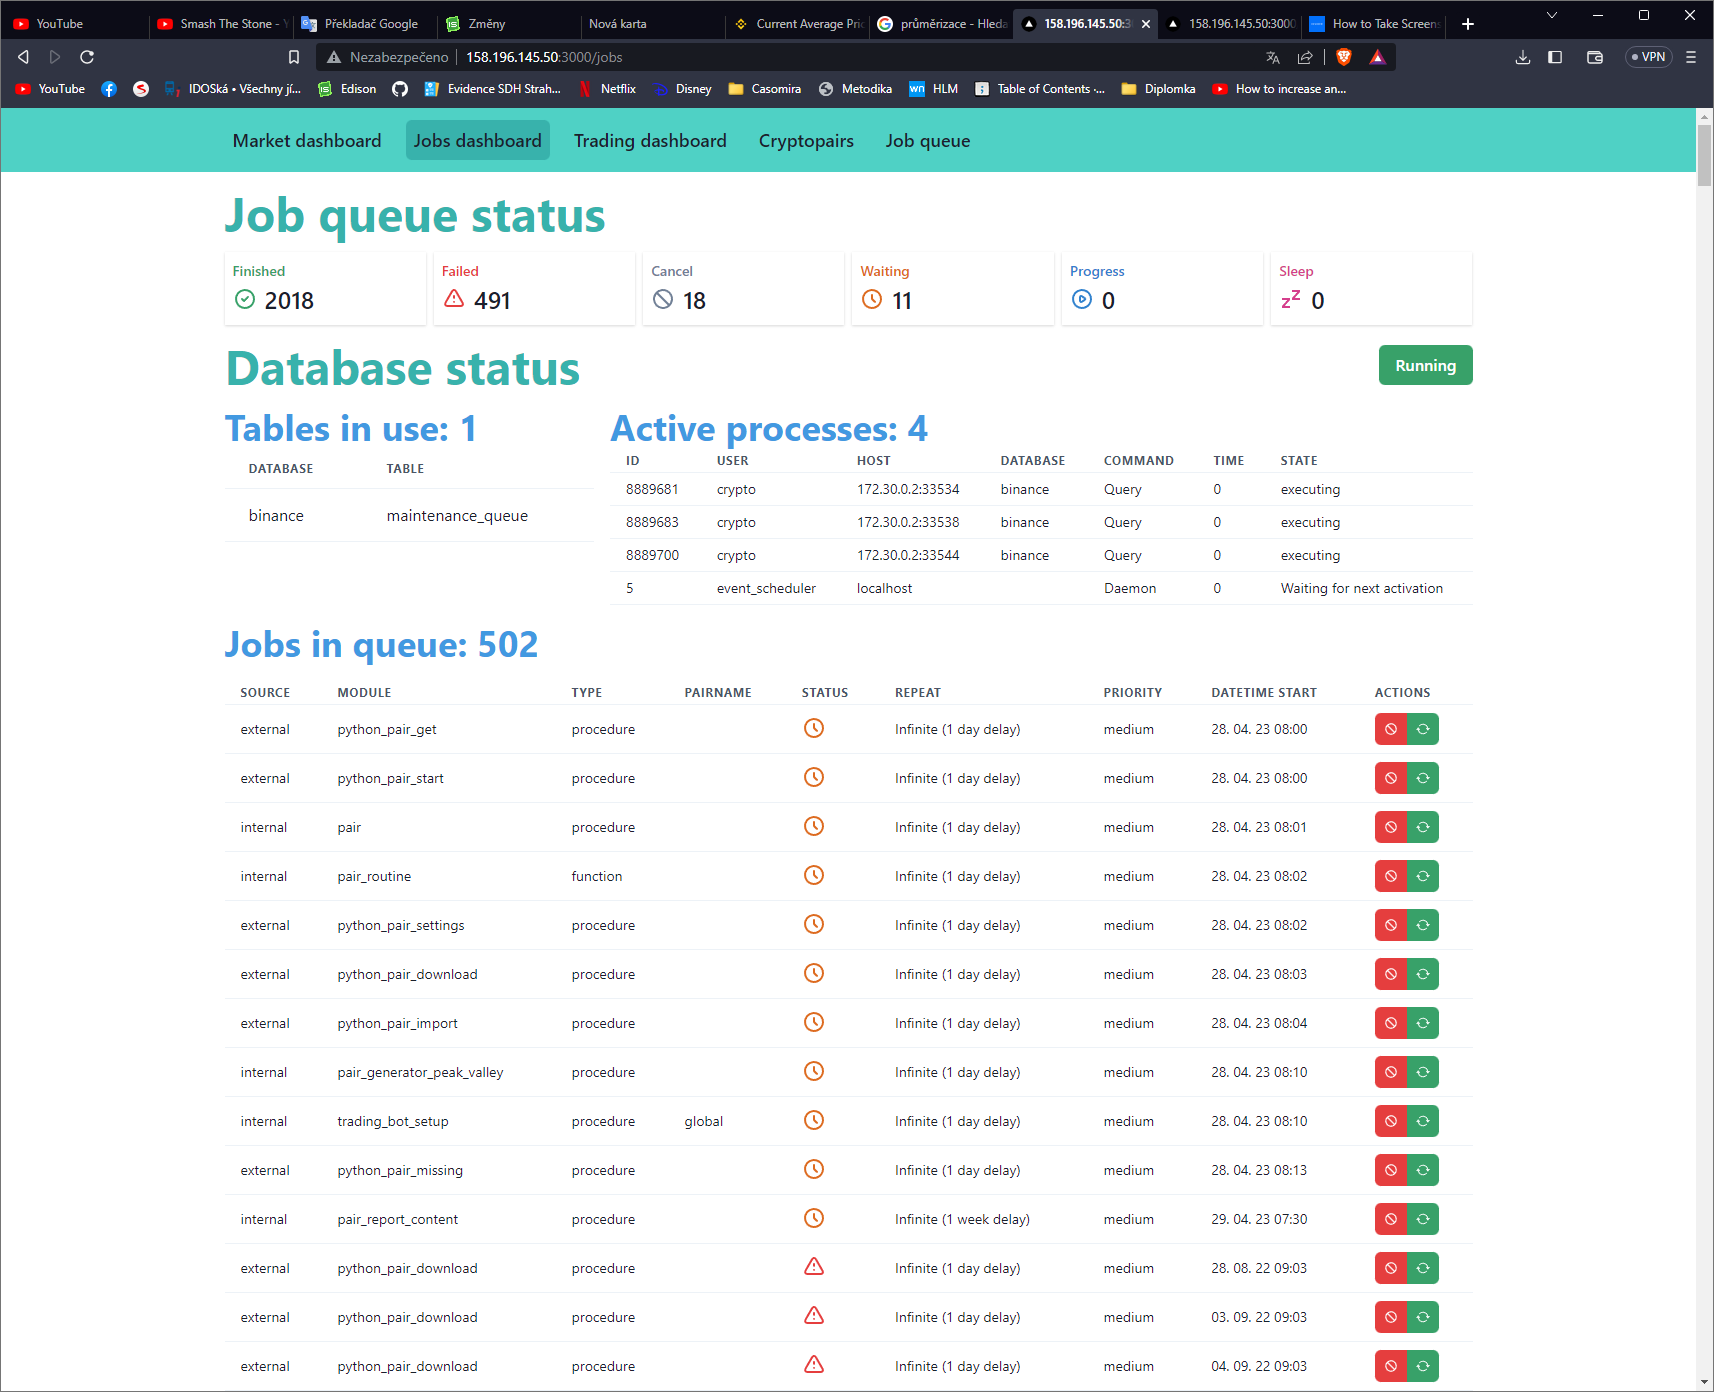
\includegraphics[width=0.6\textwidth]{Figures/web/jobs-dashboard.png}
    \caption{Stránka zobrazující stav databáze a procesů}
    \label{fig:web:jobs-dashboard}
\end{figure}

\begin{figure}[b]
    \centering
    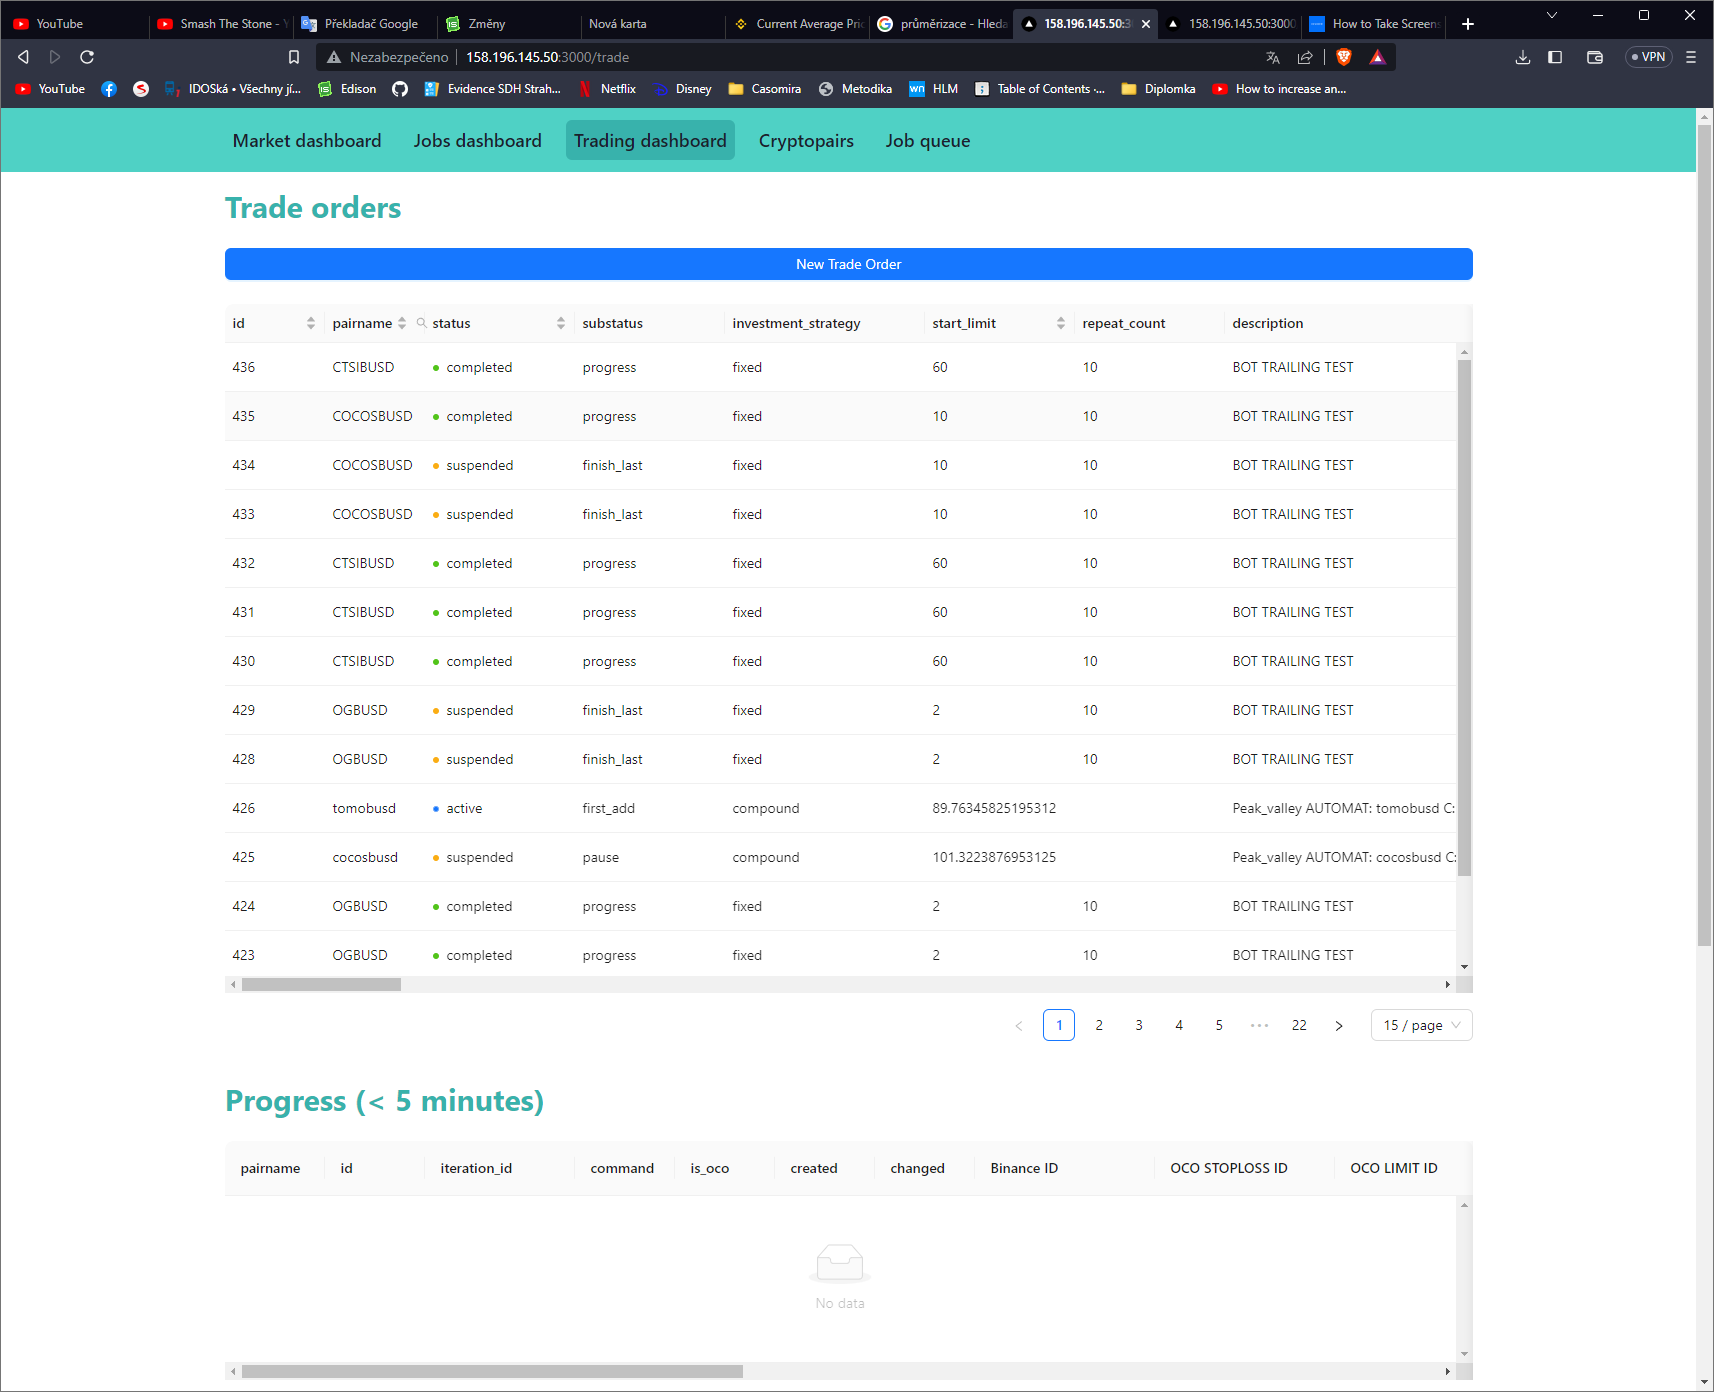
\includegraphics[width=0.6\textwidth]{Figures/web/trade-dashboard.png}
    \caption{Stránka zobrazující stav obchodních příkazů}
    \label{fig:web:trade-dashboard}
\end{figure}

\begin{figure}[b]
    \centering
    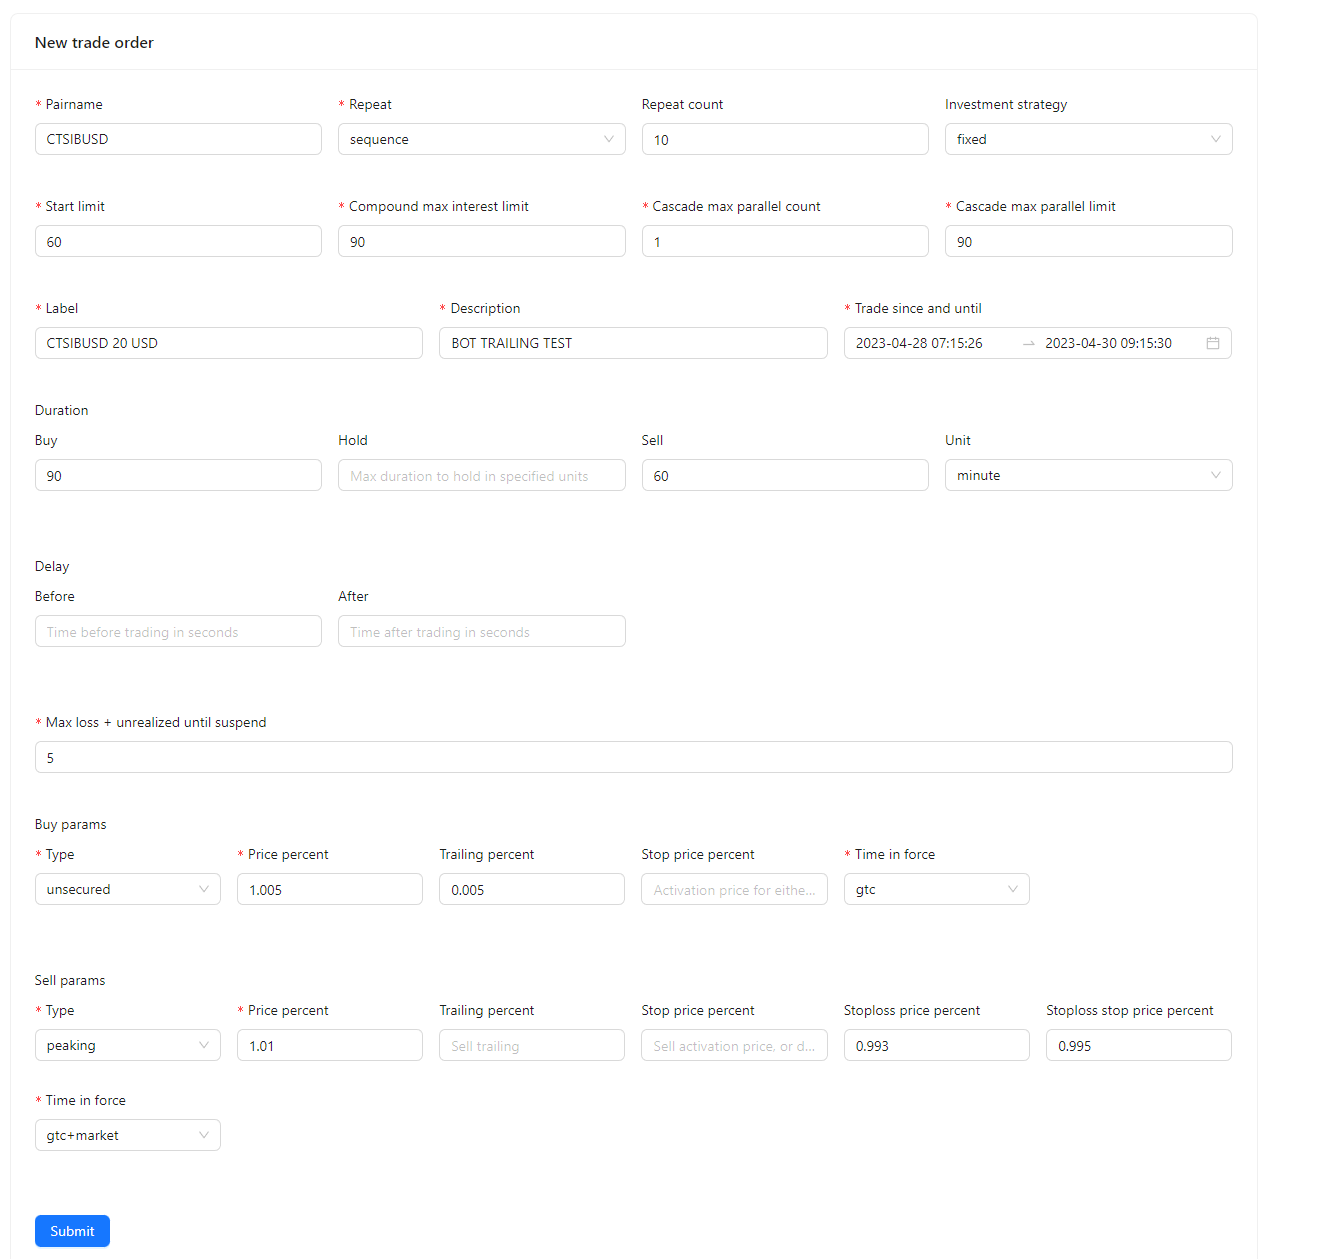
\includegraphics[width=0.6\textwidth]{Figures/web/new-order.png}
    \caption{Formulář pro zadání nového obchodního příkazu kryptobota}
    \label{fig:web:new-order}
\end{figure}

\begin{figure}[b]
    \centering
    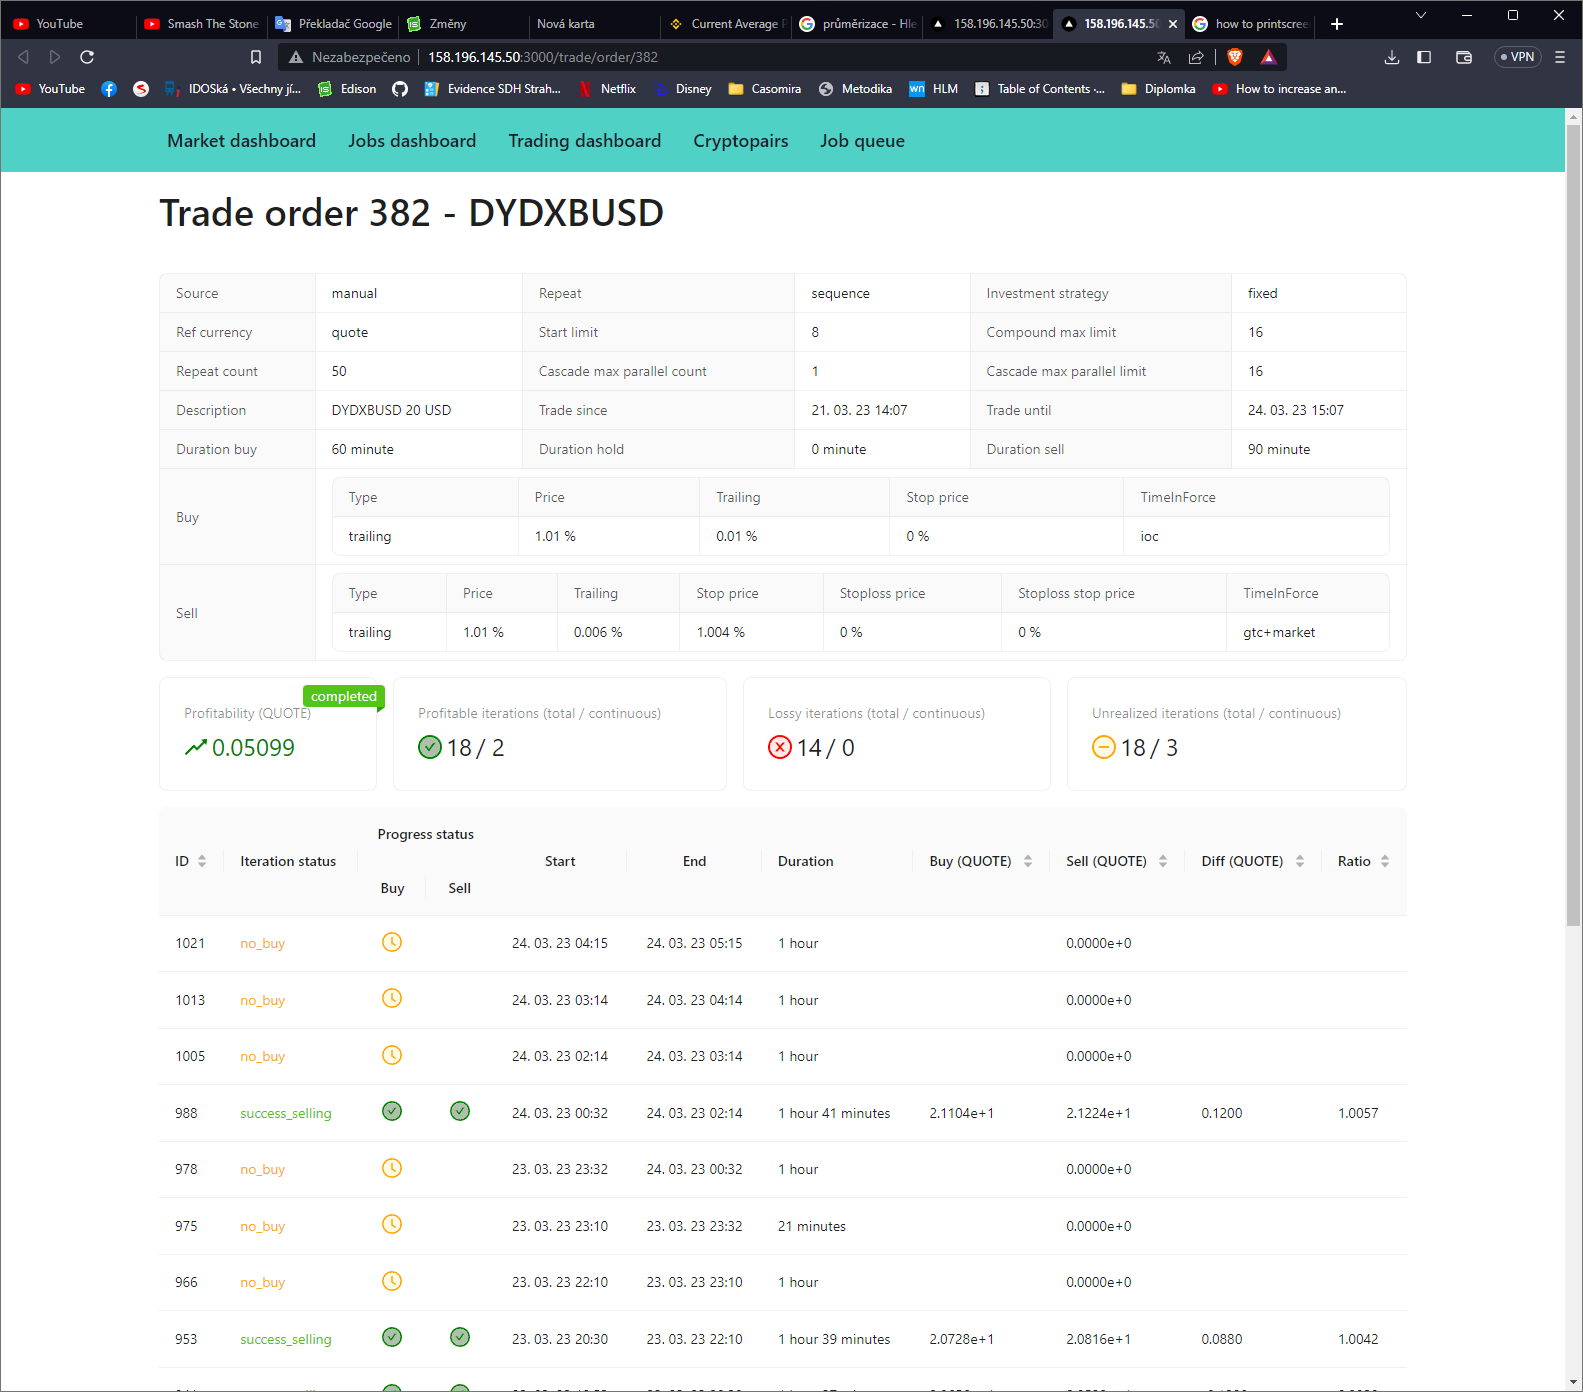
\includegraphics[width=0.6\textwidth]{Figures/web/trade-order.png}
    \caption{Výsledky obchodního příkazu}
    \label{fig:web:trade-order}
\end{figure}

\begin{figure}[ht]
    \centering
    \subfloat[\centering Nastavení obchodního příkazu]{{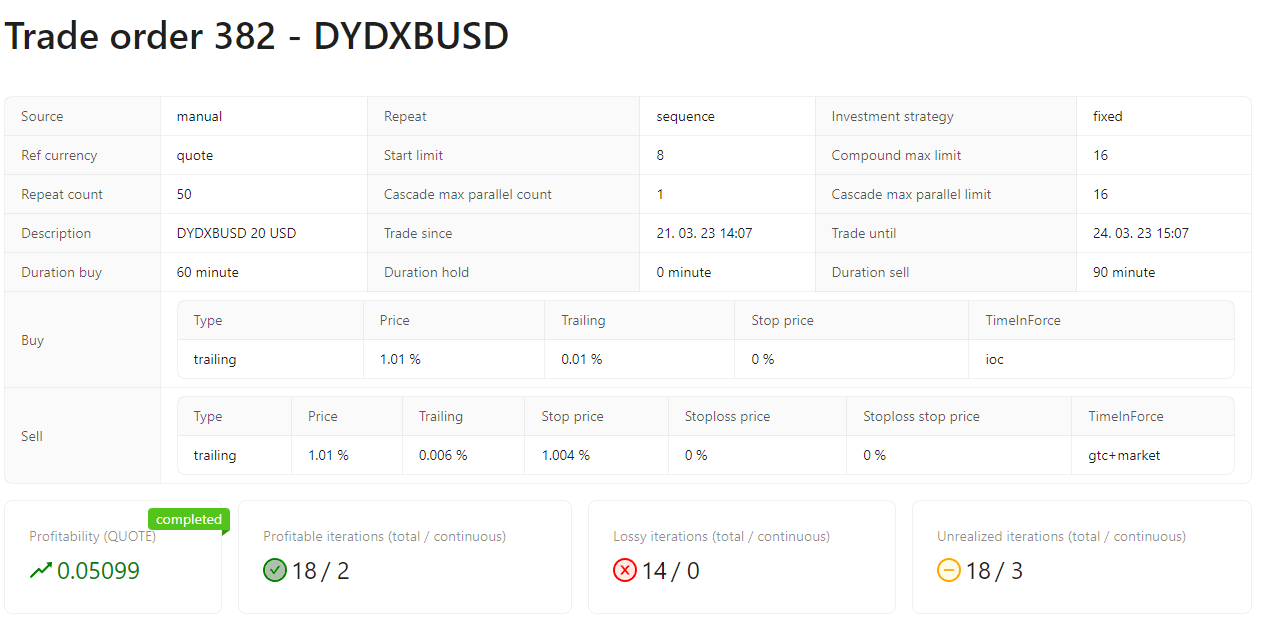
\includegraphics[width=0.45\textwidth]{Figures/web/trade-order-detail-desc.png}}\label{subfig:web:desc}}
    \qquad
    \subfloat[\centering Průběh iterací]{{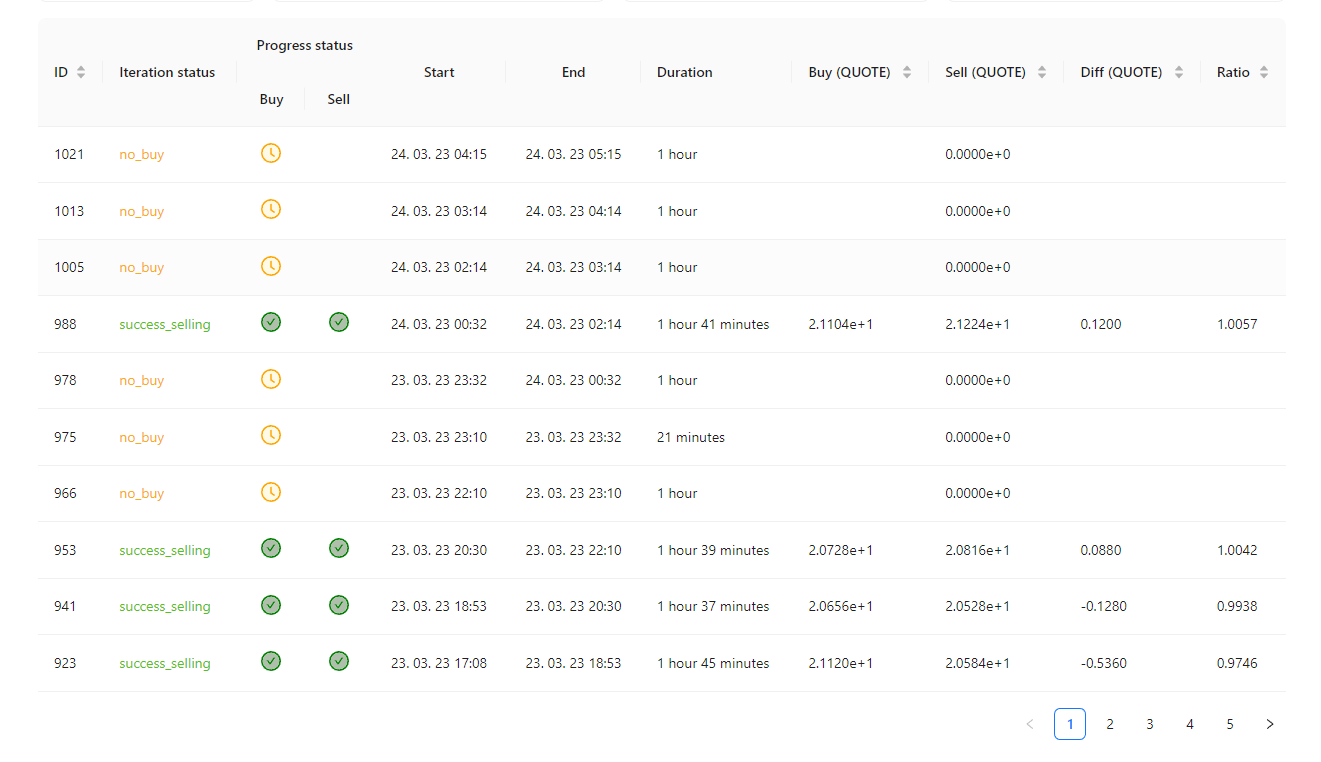
\includegraphics[width=0.45\textwidth]{Figures/web/trade-order-detail-iterations.png}}\label{subfig:web:iterations}}

    \subfloat[\centering Svíčkový graf s anotacemi průběhu iterací]{{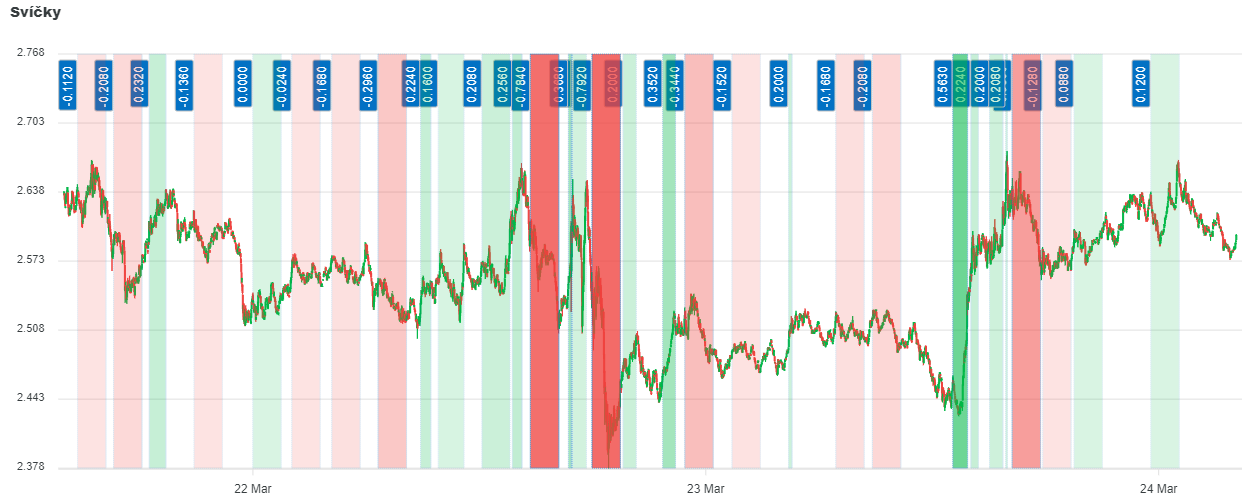
\includegraphics[width=0.8\textwidth]{Figures/web/trade-order-detail-candles.png}}\label{subfig:web:candles}}
    \caption{Detaily stránky výsledků obchodního příkazu}
    \label{fig:web:trade-order-details}
\end{figure}

\section{Možná budoucí vylepšení}
Potenciál možných rozšíření je veliký. Implementace technické analýzy se může nadále rozšiřovat o další indikátory, jako je například MACD. Tyto indikátory lze počítat na aktuálních datech získávané z burzy.
Kryptobot by tak mohl být rozšířen a dělat chytřejší rozhodnutí o tom, zda je opravdu nejlepší chvíle zaslání obchodního příkazu nebo se jedná o falešný trend.

Dalším nabízejícím se rozšířením je napojení na více kryptoměnových burz. Aktuálně je kryptobot schopen obchodovat pouze na jedné burze. Nicméně na ni není plně vázaný a což proces napojení na další
burzy značně zjednoduše.

Fundamentální analýza má taktéž potenciál na vylepšení kryptobota. Jak pozitivní, tak i negativní zprávy ohledně kryptoměn mohou ovlivňovat jejich tržní hodnotu. Kolísání této hodnoty nabízí možnost
výdělku.

Vzhledem k rozsáhlé problematice automatizovaného obchodování je množina vylepšení velká. Využít by šlo i technik strojového učení k detekci trendů nebo grafových vzorů.
Takto pokročilá vylepšení by už ale vyžadovala mnohem delší expertizu

    {\iffalse}
\begin{center}
    \small
    \begin{longtable}{ |l|c|c|p{0.3\linewidth}| }
        \hline
        Sloupec TOT                           & View                      & Příklad             & Poznámka                                                     \\
        \hline                                &                           &                     &                                                              \\
        pairname                              & pairname                  & JOEBUSD             &                                                              \\
        source                                & \tikzxmark                & peak\_valley        &                                                              \\
        rank\_trading                         & \tikzxmark                & 9999                &                                                              \\
        rank\_fundamental                     & \tikzxmark                & 9999                &                                                              \\
        rank\_total                           & \tikzxmark                & 9999                &                                                              \\
        rank\_winning\_order                  & \tikzxmark                & 1                   &                                                              \\
        market                                & \tikzxmark                & spot                & Vždy \enquote{spot}                                          \\
        type                                  & \tikzxmark                & both                & Vždy \enquote{both}                                          \\
        repeat                                & \tikzxmark                & sequence            & Vždy \enquote{sequence}                                      \\
        investment\_strategy                  & \tikzxmark                & fixed               & \enquote{fixed} nebo \enquote{compound}                      \\
        reference\_currency                   & \tikzxmark                & base                & Vždy \enquote{base}                                          \\
        start\_limit                          & all\_vol\_no\_trades\_med & 3000                & $0,6 * all\_vol\_\-no\_\-trades\_med$ pro \enquote{compound} \\
        compound\_interest\_max\_limit        & all\_vol\_no\_trades\_med & 3000                &                                                              \\
        status                                & \tikzxmark                & active              & Vždy \enquote{active}                                        \\
        repeat\_count                         & peak\_count               & first\_add          & $0,5 * peak\_count$                                          \\
        cascade\_max\_parallel\_count         & \tikzxmark                & 1                   &                                                              \\
        cascade\_max\_parallel\_limit         & \tikzxmark                & 9000                &                                                              \\
        label                                 & \tikzxmark                & JOEBUSD 20 USD      &                                                              \\
        description                           & \tikzxmark                & JOEBUSD 20 USD      &                                                              \\
        datetime\_begin                       & \tikzxmark                & 2023-03-28 12:00:00 &                                                              \\
        datetime\_end                         & \tikzxmark                & 2023-04-10 12:00:00 &                                                              \\
        duration\_buy                         & valley\_interval\_med     & 60                  &                                                              \\
        duration\_hold                        & \tikzxmark                & NULL                &                                                              \\
        duration\_sell                        & peak\_interval\_med       & 60                  &                                                              \\
        duration\_unit                        & \tikzxmark                & minute              & \enquote{minute, hour, day}                                  \\
        delay\_before                         & \tikzxmark                & NULL                &                                                              \\
        delay\_after                          & \tikzxmark                & NULL                &                                                              \\
        delay\_id                             & \tikzxmark                & NULL                &                                                              \\
        buy\_trigger                          & \tikzxmark                & last                & \enquote{last}                                               \\
        buy\_type                             & \tikzxmark                & trailing            & \enquote{market, limit, trailing, peaking, unsecured}        \\
        buy\_price\_value                     & \tikzxmark                & NULL                &                                                              \\
        buy\_price\_percent                   & change\_up                & 1.01                & $1 + change\_up$                                             \\
        buy\_trailing\_value                  & \tikzxmark                & NULL                &                                                              \\
        buy\_trailing\_percent                & change\_up                &                     & $change\_up$                                                 \\
        buy\_stop\_price\_value               & \tikzxmark                & NULL                &                                                              \\
        buy\_stop\_price\_percent             &                           &                     &                                                              \\
        buy\_time\_in\_force                  & \tikzxmark                & ioc                 &                                                              \\
        sell\_trigger                         & \tikzxmark                & last                & \enquote{last}                                               \\
        sell\_type                            & \tikzxmark                & trailing            & \enquote{market, limit, trailing, peaking, unsecured}        \\
        peaking\_period                       & \tikzxmark                & 30                  &                                                              \\
        sell\_price\_value                    & \tikzxmark                & NULL                &                                                              \\
        sell\_price\_percent                  & change\_down              &                     & $1 + change\_down$ nebo $1 - change\_down$                   \\
        sell\_trailing\_value                 & \tikzxmark                & NULL                &                                                              \\
        sell\_trailing\_percent               & change\_down              &                     & $change\_down$                                               \\
        sell\_stop\_price\_value              & \tikzxmark                & NULL                &                                                              \\
        sell\_stop\_price\_percent            & \tikzxmark                &                     &                                                              \\
        sell\_stoploss\_value                 & \tikzxmark                & NULL                &                                                              \\
        sell\_stoploss\_percent               & \tikzxmark                &                     &                                                              \\
        sell\_stoploss\_stop\_price\_value    & \tikzxmark                & NULL                &                                                              \\
        sell\_stoploss\_stop\_price\          & \tikzxmark                &                     &                                                              \\
        sell\_time\_in\_force                 & \tikzxmark                & gtc+market          &                                                              \\
        max\_loss\_unrealized\_until\_suspend & \tikzxmark                & 5                   &                                                              \\
        \hline
    \end{longtable}
\end{center}

\begin{center}
    \small
    \begin{longtable}{ |l|c|c|c|p{0.45\linewidth}| }
        \hline
        Sloupec                            & TOT        & TO         & Typ      & Popis                                                                                             \\
        \hline
        id                                 & \tikzcmark & \tikzcmark & int      & primární klíč                                                                                     \\
        pairname                           & \tikzcmark & \tikzcmark & varchar  & název kryptoměnového páru                                                                         \\
        source                             & \tikzcmark & \tikzcmark & enum     & Odkud se vzala doporučení (manual, peak\_valley)                                                  \\
        rank\_trading                      & \tikzcmark & \tikzcmark & int      & Hodnocení obchodování                                                                             \\
        rank\_fundamental                  & \tikzcmark & \tikzcmark & int      & Hodnocení fundamentu                                                                              \\
        rank\_total                        & \tikzcmark & \tikzcmark & int      & Celkové hodnocení pravidla pro obchodování,                                                       \\
        rank\_winning\_order               & \tikzcmark & \tikzcmark & int      & Vítězné pořadí pro doporučení (1 = nejlepší)                                                      \\
        market                             & \tikzcmark & \tikzcmark & enum     & Trh k obchodování (spot, futures)                                                                 \\
        type                               & \tikzcmark & \tikzcmark & enum     & Strana obchodu (buy, sell, both)                                                                  \\
        repeat                             & \tikzcmark & \tikzcmark & enum     & Opakování obchodu (once, sequence, cascade)                                                       \\
        investment\_strategy               & \tikzcmark & \tikzcmark & enum     & Investiční strategie (fixed, compound)                                                            \\
        reference\_currency                & \tikzcmark & \tikzcmark & enum     & Referenční měna (base, quote)                                                                     \\
        start\_limit                       & \tikzcmark & \tikzcmark & double   & Investovaná částka (pro fixed, pro compound pouze první investice)                                \\
        compound\_interest\_max\_limit     & \tikzcmark & \tikzcmark & double   & Maximální investovaná částka pro strategii compound (medián)                                      \\
        status                             & \tikzcmark & \tikzcmark & enum     & Status doporučení (active, suspended, cancelled, blocked)                                         \\
        substatus                          & \tikzxmark & \tikzcmark & enum     & Podrobnější status pro trade\_order (first\_add, progress, finish\_last, pause)                   \\
        repeat\_count                      & \tikzcmark & \tikzcmark & int      & Maximální počet iterací pro trade\_order                                                          \\
        cascade\_max\_parallel\_count      & \tikzcmark & \tikzcmark & int      & Maximální počet aktivních iterací v kaskádě                                                       \\
        cascade\_max\_parallel\_limit      & \tikzcmark & \tikzcmark & double   & Maximální investovaná částka aktivních iterací v kaskádě                                          \\
        label                              & \tikzcmark & \tikzcmark & varchar  & Označení                                                                                          \\
        description                        & \tikzcmark & \tikzcmark & varchar  & Popis                                                                                             \\
        datetime\_begin                    & \tikzcmark & \tikzcmark & datetime & Začáteční datum obchodování                                                                       \\
        datetime\_end                      & \tikzcmark & \tikzcmark & datetime & Konečné datum obchodování                                                                         \\
        duration\_buy                      & \tikzcmark & \tikzcmark & int      & Maximální doba pro nákup                                                                          \\
        duration\_hold                     & \tikzcmark & \tikzcmark & int      & Doba pro držení pozice                                                                            \\
        duration\_sell                     & \tikzcmark & \tikzcmark & int      & Maximální doba pro prodej                                                                         \\
        duration\_unit                     & \tikzcmark & \tikzcmark & enum     & Jednotka pro dobu prodeje/nákupu (minute, hour, day)                                              \\
        delay\_before                      & \tikzcmark & \tikzcmark & int      & Prodleva před zahájením iterace (ve vteřinách)                                                    \\
        delay\_after                       & \tikzcmark & \tikzcmark & int      & Prodleva po ukončení iterace (ve vteřinách)                                                       \\
        delay\_id                          & \tikzcmark & \tikzcmark & int      & Odkaz na pokročilejší pravidla prodlev                                                            \\
        buy\_trigger                       & \tikzcmark & \tikzcmark & enum     & Typ určující cenu nákupu pro spot/futures trh                                                     \\
        buy\_type                          & \tikzcmark & \tikzcmark & enum     & Typ nákupního příkazu (market, limit, trailing, peaking, unsecured)                               \\
        buy\_price\_value                  & \tikzcmark & \tikzcmark & double   & Cenová hodnota pro nákupní příkaz                                                                 \\
        buy\_price\_percent                & \tikzcmark & \tikzcmark & double   & Procento od aktuálního kurzu páru pro nákupní příkaz (tzn. 1.01 je 1 \% nahoru od kurzu)          \\
        buy\_trailing\_value               & \tikzcmark & \tikzcmark & double   & Cena, na kterou musí trailing vystoupat                                                           \\
        buy\_trailing\_percent             & \tikzcmark & \tikzcmark & double   & Procento trailing změny                                                                           \\
        buy\_stop\_price\_value            & \tikzcmark & \tikzcmark & double   & Aktivační cena                                                                                    \\
        buy\_stop\_price\_percent          & \tikzcmark & \tikzcmark & double   & Procento od aktuálního kurzu páru pro aktivační příkaz při nákupu                                 \\
        buy\_time\_in\_force               & \tikzcmark & \tikzcmark & enum     & Parametr pro expiraci nákupního příkazu (gtc, ioc, fok)                                           \\
        sell\_trigger                      & \tikzcmark & \tikzcmark & enum     & Typ určující cenu prodeje pro spot/futures trh                                                    \\
        sell\_type                         & \tikzcmark & \tikzcmark & enum     & Typ prodejního příkazu (market, limit, trailing, peaking, unsecured)                              \\
        peaking\_period                    & \tikzcmark & \tikzcmark & int      & Jak často má probíhat kontrola pro peaking (ve vteřinách)                                         \\
        sell\_price\_value                 & \tikzcmark & \tikzcmark & double   & Cenová hodnota pro prodejní příkaz                                                                \\
        sell\_price\_percent               & \tikzcmark & \tikzcmark & double   & Procento od aktuálního kurzu páru pro prodejní příkaz                                             \\
        sell\_trailing\_value              & \tikzcmark & \tikzcmark & double   & Cena, na kterou musí trailing vystoupat                                                           \\
        sell\_trailing\_percent            & \tikzcmark & \tikzcmark & double   & Procento trailing změny                                                                           \\
        sell\_stop\_price\_value           & \tikzcmark & \tikzcmark & double   & Aktivační cena                                                                                    \\
        sell\_stop\_price\_percent         & \tikzcmark & \tikzcmark & double   & Procento od aktuálního kurzu páru pro aktivační příkaz při prodeji                                \\
        sell\_stoploss\_value              & \tikzcmark & \tikzcmark & double   & Limitní stoploss cena, pokud je zadána, použije se OCO příkaz                                     \\
        sell\_stoploss\_percent            & \tikzcmark & \tikzcmark & double   & Procento od aktuálního kurzu pro stoploss cenu, pokud je zadána, použije se OCO příkaz            \\
        sell\_stoploss\_stop\_price\_value & \tikzcmark & \tikzcmark & double   & Aktivační cena pro stoploss                                                                       \\
        sell\_stoploss\_stop\_price\       & \tikzcmark & \tikzcmark & double   & Procento od aktuálního kurzu pro aktivační cenu pro stoploss                                      \\
        sell\_time\_in\_force              & \tikzcmark & \tikzcmark & enum     & Parametr pro expiraci nákupního příkazu (gtc, ioc, fok, gtc+market)                               \\
        current\_volume                    & \tikzxmark & \tikzcmark & double   & Aktuálně obchodované množství (investiční strategie \enquote{compound})                           \\
        profit\_volume\_last               & \tikzcmark & \tikzcmark & double   & Kolik vydělal (prodělal) poslední obchod                                                          \\
        profit\_volume\_total              & \tikzcmark & \tikzcmark & double   & Kolik celkem bylo vyděláno dané měny                                                              \\
        profit\_percent\_last              & \tikzcmark & \tikzcmark & double   & Procento zisku (ztráty) za poslední obchod                                                        \\
        profit\_percent\_total             & \tikzcmark & \tikzcmark & double   & Celkové procento zisku (ztráty)                                                                   \\
        profit\_count\_continuous          & \tikzcmark & \tikzcmark & int      & Počet po sobě provedených ziskových iterací                                                       \\
        profit\_count\_total               & \tikzcmark & \tikzcmark & int      & Celkový počet provedených ziskových iterací                                                       \\
        loss\_count\_continuous            & \tikzcmark & \tikzcmark & int      & Počet po sobě provedených prodělečných iterací                                                    \\
        loss\_count\_total                 & \tikzcmark & \tikzcmark & int      & Celkový počet provedených prodělečných iterací                                                    \\
        unrealized\_count\_continuous      & \tikzcmark & \tikzcmark & int      & Počet po sobě provedených neprovedených iterací                                                   \\
        unrealized\_count\_total           & \tikzcmark & \tikzcmark & int      & Celkový počet provedených neprovedených iterací                                                   \\
        max\_loss\_unrealized\_until\      & \tikzcmark & \tikzcmark & int      & Maximální počet po sobě jdoucích neprovedených + prodělečných iterací pro zastavení trade\_orderu \\
        profit\_percent\_last\_5           & \tikzcmark & \tikzcmark & double   & Procento zisku (ztráty) za posledních 5 obchodů                                                   \\
        suspend\_resumed\_total            & \tikzcmark & \tikzxmark & int      & Počet kolikrát byl TOT aktivován ze stavu \enquote{suspended} do stavu \enquote{active}           \\
        created                            & \tikzcmark & \tikzcmark & datetime & Kdy byl záznam vytvořen                                                                           \\
        changed                            & \tikzcmark & \tikzcmark & datetime & Kdy byl naposled záznam změněn.                                                                   \\
        \hline
        \caption{Porovnání tabulky trade\_order\_template a trade\_order}
    \end{longtable}
\end{center}

{\fi}
\endinput